%%%%%%%% ICML 2018 EXAMPLE LATEX SUBMISSION FILE %%%%%%%%%%%%%%%%%
\documentclass{article}


% hyperref makes hyperlinks in the resulting PDF.
% If your build breaks (sometimes temporarily if a hyperlink spans a page)
% please comment out the following usepackage line and replace
% \usepackage{icml2018} with \usepackage[nohyperref]{icml2018} above.
\usepackage[draft]{hyperref}

% Attempt to make hyperref and algorithmic work together better:
%\newcommand{\theHalgorithm}{\arabic{algorithm}}

% Use the following line for the initial blind version submitted for review:
\usepackage{icml2018}

% If accepted, instead use the following line for the camera-ready submission:
%\usepackage[accepted]{icml2018}

% The \icmltitle you define below is probably too long as a header.
% Therefore, a short form for the running title is supplied here:
\icmltitlerunning{CCP-IRL}

% HACK REMOVE
%\usepackage[showframe]{geometry}% http://ctan.org/pkg/geometry

\usepackage[utf8]{inputenc}
\usepackage{authblk}

\usepackage{icml2018}  %Required
\usepackage{times}  %Required
\usepackage{helvet}  %Required
\usepackage{courier}  %Required
\usepackage{url}  %Required
\usepackage{graphicx}  %Required
\usepackage{microtype}
\usepackage{subfigure}
\usepackage{booktabs} % for professional tables

\usepackage[T1]{fontenc}    % use 8-bit T1 fonts
\usepackage{amsfonts}       % blackboard math symbols
\usepackage{amsmath,amssymb}       % blackboard math symbols
\usepackage{nicefrac}       % compact symbols for 1/2, etc.
\usepackage{microtype}      % microtypography
\usepackage{bm}
\usepackage{algorithm}% http://ctan.org/pkg/algorithms
\usepackage{algorithmic}
%\usepackage{algpseudocode}% http://ctan.org/pkg/algorithmicx

%PDF Info Is Required:
\icmltitlerunning{CCP-IRL}

% \author[1]{Mohit Sharma}
% \author[1]{Kris M. Kitani}
% \affil[1]{Robotics Institute, Carnegie Mellon University}
% \affil[1]{\texttt{\{mohits1, kkitani\}@cs.cmu.edu}}
% \author[]{Joachim Groeger}
% %\affil[2]{Amazon.com}
% \affil[2]{\texttt{jrg@joachimgroeger.com}}


% \pdfinfo{
% /Title (Inverse Reinforcement Learning with Conditional Choice Probabilities)
% /Author (
%     Mohit Sharma, 
%     %\texttt{mohits1@andrew.cmu.edu}
%     %\and
%     Kris M. Kitani, 
%     %\texttt{kkitani@cs.cmu.edu}
%     %\and
%     Joachim Groeger
%     %\texttt{joachimgroeger@gmail.com})
% }

% === Kris' Macros === %
\usepackage{mathtools}
\usepackage{bm}
\renewcommand{\vec}[1]{\mbox{\bm{$#1$}}}
\def\argmax{\mathop{\rm arg\,max}}
\def\argmin{\mathop{\rm arg\,min}}

% === Mohit's Macros === %
\newcommand{\overbar}[1]{\mkern 1.5mu\overline{\mkern-1.5mu#1\mkern-1.5mu}\mkern 1.5mu}
\def\MSHangBox#1{%^
\begin{minipage}[t]{\textwidth}% Top-hanging minipage, will align on
			       % bottom of first line
\begin{tabbing} % tabbing so that minipage shrinks to fit
~\\[-\baselineskip] % Make first line zero-height
#1 % Include user's text
\end{tabbing}%^
\end{minipage}} % can't allow } onto next line, as {WIDEBOX}~x will not tie.

\usepackage{color}
\definecolor{purple}{rgb}{0.58,0,0.83}
\definecolor{red}{rgb}{1.0,0,0}
\definecolor{blue}{rgb}{0,1.0,0}
\definecolor{green}{rgb}{0,0,1.0}

\begin{document}

\twocolumn[
\icmltitle{Inverse Reinforcement Learning with \\ Conditional Choice Probabilities}]

% It is OKAY to include author information, even for blind
% submissions: the style file will automatically remove it for you
% unless you've provided the [accepted] option to the icml2018
% package.

% List of affiliations: The first argument should be a (short)
% identifier you will use later to specify author affiliations
% Academic affiliations should list Department, University, City, Region, Country
% Industry affiliations should list Company, City, Region, Country

% You can specify symbols, otherwise they are numbered in order.
% Ideally, you should not use this facility. Affiliations will be numbered
% in order of appearance and this is the preferred way.
\icmlsetsymbol{equal}{*}

\begin{icmlauthorlist}
\icmlauthor{Aeiau Zzzz}{equal,to}
\icmlauthor{Bauiu C.~Yyyy}{equal,to,goo}
\icmlauthor{Cieua Vvvvv}{goo}
\icmlauthor{Iaesut Saoeu}{ed}
\icmlauthor{Fiuea Rrrr}{to}
\icmlauthor{Tateu H.~Yasehe}{ed,to,goo}
\icmlauthor{Aaoeu Iasoh}{goo}
\icmlauthor{Buiui Eueu}{ed}
\icmlauthor{Aeuia Zzzz}{ed}
\icmlauthor{Bieea C.~Yyyy}{to,goo}
\icmlauthor{Teoau Xxxx}{ed}
\icmlauthor{Eee Pppp}{ed}
\end{icmlauthorlist}

\icmlaffiliation{to}{}
\icmlaffiliation{goo}{}
\icmlaffiliation{ed}{}

\icmlcorrespondingauthor{}{}
\icmlcorrespondingauthor{}{}

% You may provide any keywords that you
% find helpful for describing your paper; these are used to populate
% the "keywords" metadata in the PDF but will not be shown in the document
\icmlkeywords{Machine Learning, ICML}

\vskip 0.3in


% this must go after the closing bracket ] following \twocolumn[ ...

% This command actually creates the footnote in the first column
% listing the affiliations and the copyright notice.
% The command takes one argument, which is text to display at the start of the footnote.
% The \icmlEqualContribution command is standard text for equal contribution.
% Remove it (just {}) if you do not need this facility.

%\printAffiliationsAndNotice{}  % leave blank if no need to mention equal contribution
%\printAffiliationsAndNotice{\icmlEqualContribution} % otherwise use the standard text.

\begin{abstract}
We make an important connection to existing results in econometrics to describe an alternative formulation of inverse reinforcement learning (IRL). In particular, we describe an algorithm using Conditional Choice Probabilities (CCP), which are maximum likelihood estimates of the policy estimated from expert demonstrations, to solve the IRL problem. Using the language of structural econometrics, we re-frame the optimal decision problem and introduce an alternative representation of value functions due to \cite{hotz}. In addition to presenting the theoretical connections that bridge the IRL literature between Economics and Robotics, the use of CCPs also has the practical benefit of reducing the computational cost of solving the IRL problem. Specifically, under the CCP representation, we show how one can avoid repeated calls to the dynamic programming subroutine typically used in model-based IRL. We show via extensive experimentation on standard IRL benchmarks that CCP-IRL is able to outperform MaxEnt-IRL, with as much as a 5x speedup and without compromising on the quality of the recovered reward function.
\end{abstract} 

\section{Introduction}

The problem of extracting the reward function of a task given observed optimal behavior has been studied in parallel in both robotics and economics. In robotics this literature is collected under the heading "Inverse Reinforcement Learning" (IRL), \cite{Ng2000, abbeel2004apprenticeship}. The aim here is to learn a reward function that best explains demonstrations of expert behavior so that a robotic system can reproduce expert like behavior. In economics this literature is referred to as "structural econometrics" \cite{miller, pakes, rust_gmc}. Estimates are used to better understand human decision making and to simulate optimizing responses to changes in the environment, such as new constraints on choices. Although both fields developed in parallel, they are similar in that both seek to uncover a latent reward function of an underlying Markov Decision Process (MDP). In this work, we make important connections between both fields.

% Both of the fields are similar in that both seek to uncover a \emph{latent} reward function of an underlying Markov Decision Process (MDP).
% Although both fields developed in parallel there has been very limited knowledge transfer between them. To alleviate this we make the connection between these two fields more explicit. We uncover different problem formulations which give rise to similar algorithms. Specifically, we show how the softmax value function in \cite{ziebart} is exactly similar to the ex-ante value function in \cite{rust_gmc} under Type-1 extremum assumption.

One of the main challenges in IRL is the large computational complexity of modern algorithms \cite{ziebart, Ratliff2006}. To infer the reward function of the underlying MDP, one must \textit{repeatedly} solve this MDP at every step of a reward parameter optimization scheme. The MDP solution, which is typically characterized by a value function, requires a computationally expensive Dynamic Programming (DP) procedure. Unfortunately, solving this DP step repeatedly makes IRL algorithms computationally prohibitive.  

This problem of computational complexity has also been studied in economics \cite{hotz, su2012constrained, aguirregabiria2002swapping}. Among the many works, Conditional Choice Probability (CCP) estimators \cite{hotz} are particularly interesting because of their computational efficiency.
CCP estimators use CCP values to estimate the reward function of the MDP.
The CCP values specify the optimal action for a state and are estimated from expert demonstrations. These estimators are computationally efficient, since they avoid the repeated computation of the DP step by using an alternative representation of the MDP's value function. As shown by \cite{magnac}, the CCP-IRL framework also enables us to estimate the reward function non-parametrically. We derive this result in the appendix.\footnote{\cite{klein2012inverse} derive an alternative framework that also avoids repeated solution of the DP. However, they are restricted to considering reward functions that can be expressed in linear form. The CCP framework provides greater flexibilty and does not rely on linearity to reduce computation.} Moreover, there are further benefits when considering non-stationary environments, discussed in \cite{arcidiacono2014nonstationary}.

In this work we introduce Conditional Choice Probability IRL (CCP-IRL) by incorporating CCPs into IRL. We leverage results from \cite{rust_gmc, hotz, magnac} to formulate an estimation routine for the reward function with CCPs, that avoids repeated calls to the solver of the full dynamic decision problem. We test the CCP-IRL algorithm on multiple different IRL benchmarks and compare the results to the state-of-the-art IRL algorithm, MaxEnt-IRL \cite{ziebart}. In our experiments, we show that with CCP-IRL we can achieve up to 10$\times$ speedup without affecting the quality of the inferred reward function. Further, this speedup holds across large state spaces and increases for complex problems, such as, problems where value iteration takes much longer to converge. 


To summarize our contributions, in this work we make an important connection between economics and robotics to uncover different problem formulations that result in similar algorithms. We then use this connection to leverage the literature of conditional choice probabilities and propose a new IRL algorithm called CCP-IRL. We test the CCP-IRL algorithm on multiple different IRL benchmarks and show that we get an order of magnitude speedup. Further, we also discuss how the CCP approach is applicable to other important areas in IRL research. We believe our work will help researchers from both fields to leverage literature from other field and thus lead to more knowledge transfer.


%==========================================================%
\section{Preliminaries}

In this section, we first introduce the MDP formulation as used in the econometrics literature under the name "Dynamic Discrete Choice Model". Following this, we show how the optimality equation is formulated under these assumptions, and how the resulting optimization problems can be related to traditional IRL algorithms.

\subsection{Dynamic Discrete Choice Model}

A dynamic discrete choice (DDC) model (\emph{i.e.}, a discrete Markov decision process with action shocks) is defined as a tuple $(\mathcal{X,A}, T,r,\mathcal{E},F)$. 
We assume a discrete state space, to avoid technical machinery out of the scope of this paper, although this is not strictly necessary.
$\mathcal{X}$ is a countable set of states with a cardinality of $|\mathcal{X}|$. $\mathcal{A}$ is a finite set of actions with cardinality $|\mathcal{A}|$. $T$ is the transition function where $T(x'|x,a)$ is the probability of reaching state $x'$ given current state $x$ and action $a$. The reward function $r$ is a mapping $r:\mathcal{A}\times\mathcal{X}\rightarrow \mathbb{R}$.

Different from MDPs typically used in RL, each action also has a "payoff-shock" associated with it that enters payoffs additively.
The motivation for this perturbation originates from the discrete choice literature \cite{mcfadden1973conditional} on static models as a way of reconciling why numerous economic agents with identical observed characteristics make different decisions to each other. Rather than assuming the agents are indifferent between all the decisions,
%that at least one of them takes (which might cover the choice set)
an alternative assumption is that there is an additional characteristic pertinent for decision making that the modeller does not observe. The simplest of way of modeling this unobserved characteristic is to treat it as an independent, identically distributed random variable, one for each element in the choice set. Adding a payoff-shock to each choice at every decision node in DDC models is the dynamic analogue to escape a similar lacuna.
This vector of shocks is denoted $\vec{\epsilon} = [ \epsilon_{1} \cdots \epsilon_{|\mathcal{A}|} ]$ and $\vec{\epsilon}\in \mathbb{R}^{|\mathcal{A}|}$. Total rewards for action $a \in \mathcal{A}$ in state $x \in \mathcal{X}$ are therefore given by:
\begin{eqnarray}
r(a,x)+\epsilon_a
\end{eqnarray}
A shock value $\epsilon_a\in\mathbb{R}$ is often assumed to be distributed according to a Gumbel or Type 1 Extreme Value (TIEV) distribution,
\begin{align}
F(\epsilon_a)=e^{-e^{-\epsilon_a}}
\end{align}
We will see that the use of a TIEV distribution is numerically convenient for the following derivations. However, alternative algorithms can be derived for other functional forms. Each shock $\epsilon_a$ is independently and identically drawn from $F(\epsilon_a)$. This ensures that state transitions are conditionally independent. All serial dependence between $\epsilon_{t}$ and $\epsilon_{t+1}$ is transmitted through $x_{t+1}$. \cite{rust_theory} proves the existence of optimal stationary policies in this setting.

\subsection{Bellman Optimality Equation Derivation}

Consider a system currently in state $(x_t,\vec{\epsilon}_t)$, where $\vec{\epsilon}_t$ is a vector of shock values. The decision problem is to select the action that maximizes the payoff:
\begin{align}
\begin{split}
V(x_t,\vec{\epsilon}_t) & = \max_{a\in\mathcal{A}} \big\{r(x_t,a)+\epsilon_{at} \\
& \qquad + \beta \cdot E_{x_{t+1},\vec{\epsilon}_{t+1}|x_t,a} \left[V(x_{t+1},\vec{\epsilon}_{t+1})\right] \big\} \\
\end{split}
\end{align} 
where $V$ is the value function, $\beta$ is the discount factor and $\epsilon_{at} \in \vec{\epsilon}_t$ is the shock value when selecting action $a$ at time $t$.


Given the conditional independence assumption of the shock variable described previously, we can separate the integration of $x_{t+1}$ and $\vec{\epsilon}$. Define the \emph{ex-ante} value function (i.e., $V$ prior to the revelation of the values of $\epsilon$) as:
\begin{eqnarray}\label{eq:def_exante}
\overline{V}(x_t)
\triangleq 
E_{\vec{\epsilon}_t} \left[ V(x_t, \vec{\epsilon}_t) \right],
\end{eqnarray}
that is, the expectation of the value function with respect to the shock distribution. Using this notation and conditional independence, we can write the original decision problem as:
% NOTE: 
% Cannot use \left \right to dynamically scale {} 
% This trick doesn't seem to work (https://tex.stackexchange.com/questions/49890/linebreak-between-left-and-right)
%
\begin{align}
\begin{split}
V(x_t,\vec{\epsilon}_t) & =\max_{a\in\mathcal{A}} \big\{ \vphantom{V} r(x_t,a)+\epsilon_{at}  \\
&  \, +\beta \cdot E_{x_{t+1}|x_t,a} \left[ \overline{V}(x_{t+1}) \right] \vphantom{r(x_t, a)} \big\}.
\nonumber
\end{split}
\end{align}


The \emph{ex-ante} value function also follows a Bellman-like equation:
\begin{align} \label{eq:exantebellman}
\begin{split}
\overline{V}(x_t) & = E_{\vec{\epsilon}_t}\Big[\max_{a\in\mathcal{A}} \big\{r(x_t,a)+\epsilon_{at} \\
& +\beta  \cdot E_{x_{t+1}|a,x_t} \left[ \overline{V}(x_{t+1}) \right] \big\}\Big]
\end{split}
\end{align}

Assuming TIEV distribution for the shock values, one obtains the following expression for the \emph{ex-ante} value functions as shown by \cite{rust_gmc}:
\begin{align} \label{eq:exanterust}
\begin{split}
\overline{V}(x_t) &=\ln\left[\sum_{a\in\mathcal{A}} \exp\left(r(x_t,a)+\beta \cdot E_{x_{t+1}|a,x_t} \left[ \overline{V}(x_{t+1}) \right] \right)\right] \\
& \qquad +\gamma,
\end{split}
\end{align}
where $\gamma$ is Euler's constant. The expectation of the maximum is equal to the average of expected value functions, conditional on choosing action $a$ with $\vec{\epsilon}$ integrated using the TIEV density. Weights in the average are given by the CCPs of choosing action $a$.

% E(max(a,b)) = Pr(a>b)E(a|a>b)+Pr(b>a) E(b|b>a)

Notice that the above is exactly the recursive representation of the Maximum Causal Entropy IOC algorithm as derived in Theorem 6.8 in \cite{ziebart_phd}. In our setting, the soft-max recursion is a consequence of Bellman's optimality principle in a setting with a separable stochastic payoff shock with a TIEV distribution, while in \cite{ziebart_phd} the authors derive the recursion from an information-theoretic perspective that enforces a maximum causal entropy distribution over trajectories.

%===============================================================%
\subsection{Conditional Choice Probability}

%We will now show how it is possible to efficiently recover the optimal value function, and consequently the underlying reward function, using the DDC model. The key insight is that the optimal value function can be directly estimated from observed state-actions pairs (Conditional Choice probabilities), observed over a set of expert demonstrations. When this assumption holds the optimal value function can be represented as a linear function of the CCPs and efficiently computed for different parameter values without solving the DP problem iteratively.

We now show how the conditional choice probabilities can be estimated from the ex-ante value function.
Since an outside observer does not have access to the shock ($\vec{\epsilon}$), the underlying deterministic policy of the expert $\sigma(a | x,\epsilon)$ is not directly measurable. However, if we average decisions across trajectories conditioned on the same state variables we are able to identify the integrated policy. We denote this integrated policy by $\sigma(a|x)\in[0,1]$, the \emph{conditional choice probability} (CCP) of an action being chosen conditioned on state $x$: 
\begin{eqnarray}
\sigma(a|x_t)\triangleq E_{\vec{\epsilon}}\left[ \mathbf{1}\{a\ \textrm{is optimal in state }x_t\}\right],
\end{eqnarray}
where $\mathbf{1}\{\}$ is the indicator function. The event in the indicator function is equivalent to the event:
\begin{align}
\begin{split}
& \left\{r(x_t,a)+\epsilon_{at}+\beta E_{x_{t+1}|a,x_t} \overline{V}(x_{t+1})\geq \right. \\
& \quad \left. r(x_t,a')+\epsilon_{a't}+\beta E_{x_{t+1}|a',x_t} \overline{V}(x_{t+1}),\ \forall a'\neq a \right\}
\end{split}
\end{align}
Expanding the expectation under the TIEV assumption on the shock variable allows CCPs to be solved in closed-form:
\begin{align} \label{eq:ccps}
\begin{split}
\sigma(a|x_t)=\frac{\exp\left(r(x_t,a)+\beta E_{x_{t+1}|x_t,a} \overline{V}(x_{t+1})\right)}{\sum_{a'\in\mathcal{A}} \exp\left(r(x_t,a')+\beta E_{x_{t+1}|x_t,a'} \overline{V}(x_{t+1})\right)}
\end{split}
\end{align}
Notice that \eqref{eq:ccps} is identical to the definition of the policy of the MaxEnt formulation in \cite{ziebart_phd}, which is derived from an entropic prior on trajectories. The CCP is derived by integrating out the TIEV shock variable. 





\section{Conditional Choice Probability - Inverse Reinforcement Learning}

Our aim in IRL is to estimate the reward function, usually parameterized $r(\theta)$, for the given MDP/R. We now show how we can leverage \textit{non-parameteric} estimates of choice conditional probabilities to efficiently estimate the parameters $\theta$ of the reward function. The key insight is that the optimal value function can be directly estimated from observed state-actions pairs (CCPs), observed over a set of expert demonstrations.
First, we look at the alternative representation of the \emph{ex-ante} value function which can be derived from CCP estimates. Following this, we see how using this alternative representation can avoid solving the original MDP problem repeatedly.
For convenience, we will write the parameterized reward function as $r_{\theta}(x)$.

\subsection{Model-based Reinforcement Learning with CCPs}

Returning to the definition of the \emph{ex-ante} value function in Equation \eqref{eq:def_exante} and \eqref{eq:exantebellman}, notice that Equation \eqref{eq:exantebellman} is similar to the state-value function definition in reinforcement learning. 
Analogously, define the integrated choice-specific value function $V_a(x_t)$ as the reward and future value as:
\begin{align}
\begin{split}
V_a(x_t) &= E_{\vec{\epsilon}_t}\left[r_{\theta}(x_t,a)+\epsilon_{at}\right.\\
&
\left.\beta\cdot E_{x_{t+1}|a,x_t} \left[ \overline{V}(x_{t+1}) \right] \right]
\end{split}
\end{align}

Hotz and Miller \yrcite{hotz} show that given \textit{consistent} CCP estimates from the data, equation \eqref{eq:exantebellman} can be estimated as,
\begin{align} \label{eq:exantebellman_2}
\begin{split}
\overline{V}(x_t) & = E_{\vec{\epsilon}_t}\Big[\sum_{a\in\mathcal{A}} \sigma(a|x_t) \big\{r_{\theta}(x_t,a)+\epsilon_{at} \\
& \qquad +\beta  \cdot E_{x_{t+1}|a,x_t} \left[ \overline{V}(x_{t+1}) \right] \big\}\Big]\\
\end{split}
\end{align}
Now, defining the expected shock given that action $a$ is optimal as $\tilde{\epsilon}(a|x_t) = E_{\vec{\epsilon}}\left( \epsilon_{at} |a\ \textrm{is optimal in state } x_t\right)$, we can rewrite \eqref{eq:exantebellman_2} as,
\begin{align} \label{eq:exantebellman_3}
\begin{split}
\overline{V}(x_t) & = \sum_{a\in\mathcal{A}} \sigma(a|x_t) \Big[r_{\theta}(x_t,a)+\tilde{\epsilon}(a|x_t) \\
& \qquad +\beta \sum_{x_{t+1}\in\mathcal{X}} T(x_{t+1}|x_t,a) \overline{V}(x_{t+1})\Big]
\end{split}
\end{align}
Hotz and Miller \yrcite{hotz} further show that $\tilde{\epsilon}(a|x_t)$ depends on CCPs and distribution of $\epsilon$ only.
To see this, notice that CCPs can be expressed as function of differences in choice specific value function, since action $a$ being optimal implies $V_a(x_t)- V_{a'}(x_t)\geq 0 \quad\forall a'\in\mathcal{A} - \{a\}$. The cornerstone of Hotz and Miller's approach is to show that this mapping between CCPs and choice specific value function is \emph{invertible}. Using this inverse mapping and assuming TIEV distribution for $\epsilon$, we get $\tilde{\epsilon}(a|x_t) = \gamma - \log \sigma(a|x_t)$.

Using this result we will now write a closed form solution for $\overline{V}(x_t)$. For this we will first stack the \emph{ex-ante} value function over all states. Doing this we get,
\begin{align} \label{eq:exantebellman_4}
    \begin{split}
    \overline{\mathbf{V}}=\sum_{a}\mathbf{S}(a) \times \left[\mathbf{R}_{\theta}(a)+\tilde{\bm{\epsilon}}(a)+\beta \mathbf{T}(a) \overline{\mathbf{V}}\right]
    \end{split}
\end{align}
where:
\begin{align}
\overline{\mathbf{V}}=\left[\begin{array}{c}\overline{V}(x_1)\\\vdots\\\overline{V}(x_{|\mathcal{X}|})\end{array}\right]
\mathbf{R}_{\theta}(a)=\left[\begin{array}{c}r_{\theta}(x_1,a)\\\vdots\\ r_{\theta}(x_{|\mathcal{X}|},a)\end{array}\right]
\end{align}
\begin{align}
\mathbf{T}(a)=\left[\begin{array}{ccc}
T(x_1|x_1,a),\dots,T(x_{|\mathcal{X}|},x_1,a)\\
\vdots\\
T(x_1|x_{|\mathcal{X}|},a),\dots,T(x_{|\mathcal{X}|},x_{|\mathcal{X}|},a)\\
\end{array}\right]
\end{align}
Similarly, writing matrices $\mathbf{S}(a) = [\sigma(a|x); x\in\mathcal{X}]$ and $\tilde{\bm{\epsilon}}(a)=[\tilde{\epsilon}(a|x); x\in\mathcal{X}]$.
Rearranging the terms in \eqref{eq:exantebellman_4},
\begin{align}
    \begin{split}
    \overline{\mathbf{V}}-\sum_{a}\mathbf{S}(a) *\left[ \beta \mathbf{T}(a) \overline{\mathbf{V}}\right]=\sum_{a}\mathbf{S}(a) *\left[ \mathbf{R}_{\theta}(a)+\tilde{\bm{\epsilon}}(a)\right]
    \end{split}
\end{align}

Defining $\lambda$ as a $1\times|\mathcal{X}|$ vector of ones, we can write the closed form solution for $\overline{\mathbf{V}}$ as,
\begin{align} \label{eq:exante_inversion}
\begin{split}
\overline{\mathbf{V}} &=\left[I-\sum_{a}(\mathbf{S}(a) \lambda) *\left[ \beta \mathbf{T}(a)  \right]\right]^{-1} \\
& \qquad \times \left[\sum_{a}\mathbf{S}(a) *\left[ \mathbf{R}_{\theta}(a)+\tilde{\bm{\epsilon}}(a)\right]\right]
\end{split}
\end{align}
Notice that the inverse matrix in \eqref{eq:exante_inversion} is similar to the inverse matrix required for value function estimation in policy evaluation. The computational complexity of solving \eqref{eq:exante_inversion} is thus equivalent to known policy evaluation algorithms.\footnote{An alternative to using \ref{eq:exante_inversion} to estimate the value function is to use monte-carlo approximation, i.e. using the CCPs and transition matrix to simulate and store future a large number of action and state paths.}

\subsection{Linear Reward Parameterization}

The above closed form equation holds in the most general case of a non-parametric reward function. Equation \eqref{eq:exante_inversion} can be further simplified for a linear reward parameterization; $r_{\theta}(x,a) = \theta^{\top} z(x,a)$, where $z(x, a)$ is a feature representation for a given state-action pair. Stacking up the feature values we define $\mathbf{Z}(a) = [z(x, a); x \in \mathcal{X}]$. As before we stack the integrated choice-specific value function to get $\mathbf{V}_a$. From \eqref{eq:exantebellman_4} we get
\begin{align} \label{eq:exante_linear}
    \begin{split}
    \mathbf{V}_a=\mathbf{R}_{\theta}(a)+\widetilde{\vec{\epsilon}}(a)+\beta \mathbf{T}(a) \sum_{a'}\mathbf{S}(a')\mathbf{V}_a'
    \end{split}
\end{align}
Since $\mathbf{R}_{\theta}(a) = \mathbf{Z}(a)^T\theta$ for linear parameters, it is easy to show that \eqref{eq:exante_linear} can be written as $\mathbf{V}_a = \hat{\mathbf{Z}}(a)^T\theta + \hat{\bm{\epsilon}}(a)$, where we define
\begin{align} \label{eq:choice_specific_Z_tilde}
\begin{split}
    \hat{\mathbf{Z}}(a) = \mathbf{Z}(a) + \beta\mathbf{T}(a)\sum_{a'}\mathbf{S}(a')\hat{\mathbf{Z}}(a') \\
    \hat{\bm{\epsilon}}(a) = \tilde{\bm{\epsilon}}(a) + \beta\mathbf{T}(a)\sum_{a'}\mathbf{S}(a')\hat{\bm{\epsilon}}(a')
\end{split}    
\end{align}
Again both $\hat{\mathbf{Z}}(a)$ and $\hat{\bm{\epsilon}}(a)$ can be estimated via backwards recursion and is computationally similar to a single policy evaluation algorithm.

In the above, we have shown how CCPs can be used to estimate a parameterized reward function. However, the CCP approach is more general and can also be used to estimate the reward functions \textit{non-parametrically}, conditional on assuming one action reward can be normalized to zero. We discuss these results in the Appendix.

\begin{figure*}[ht]
\begin{minipage}[t]{0.45\textwidth}
  %\vspace{0pt}  
  \begin{algorithm}[H]
    \caption{CCP-IRL algorithm} \label{algo:ccp_irl_algorithm}
    \begin{algorithmic}[1]
        %\Procedure{CCP-IRL}{$\mu_D,f, S, A, T, \gamma$}
        \STATE {\bfseries Input:} expert features $\mu_D$, ccp $\mathbf{S}$, transition $\mathbf{T}$, discount $\gamma$
        \STATE $\theta^{(0)} \gets$ init\_weights
        \STATE $\mathbf{M} \gets \left[\mathbf{I}-\sum_{a}(\mathbf{S}(a) \lambda) *\left[ \gamma \mathbf{T}(a)  \right]\right]^{-1}$ 
        \STATE $\tilde{\bm{\epsilon}} \gets \gamma - \log \mathbf{S}(a)$
        \FOR{$i\gets 1, n$}
            \STATE $R^{(i)} \gets \mathbf{R}(\theta^{(i)}))$
            \STATE $V^{(i)} \gets \mathbf{M} \times \sum_{a}{\mathbf{S}(a) \times \left[ R^{(i)} +\tilde{\bm{\epsilon}}\right]}$
            \STATE $\pi_{\theta}^{(i)}(a|x) \gets e^{V^{(i)}(x_a) - V^{(i)}(x)}$
            \STATE $E[\mu^{(i)}] \gets $ FORWARD PASS()
            \STATE $\theta^{(i)} \gets \theta^{(i-1)} - \alpha \times (\mu_D - E[\mu^{(i)}])$
        \ENDFOR
    \end{algorithmic}
  \end{algorithm}
\end{minipage}%
\qquad
\begin{minipage}[t]{0.45\textwidth}
  %\vspace{0pt}
  \begin{algorithm}[H]
    \caption{Forward Pass} \label{algo:forward_pass_algorithm}
    \begin{algorithmic}[1]
        \STATE {\bfseries Input:} policy $\pi_{\theta(a|x)}$
        \STATE $D^{(0)}(x) \gets P(x_i = x_{initial})$
        \FOR{$i\gets 1, n$}
            \STATE $D^{(i-1)}(x_{goal}) \gets 0$
            \STATE $D^{(i)}(x) \gets D^{(i)}(x) + \pi_{\theta}(a|x') D^{(i-1)}(x')$
        \ENDFOR
        \STATE $D(x) \gets \sum_{i}D^{(i)}(x)$ 
        \STATE \textbf{return} $D(x)$
    \end{algorithmic}
  \end{algorithm}
\end{minipage}
\end{figure*}


\subsection{Inverse Reinforcement Learning with CCPs}
We now look at how to efficiently solve the IRL problem using the above value function representation. 
We compare against MaxEnt-IRL, since, as shown above, the ex-ante value function representation is similar to MaxEnt-IRL.
MaxEnt-IRL involves estimating the parameters $\theta$ of the reward function using an iterative procedure.
At every step of the iteration, we need to estimate the value function by solving the MDP problem using an RL algorithm. Since this happens repeatedly, it can be prohibitively expensive.

In contrast, the above value function representations (\eqref{eq:exante_inversion} and \eqref{eq:exante_linear}) can be used to estimate the value function much more efficiently. To see this, notice that in \eqref{eq:exante_inversion} we can pre-calculate the inverse matrix once. Alternately, for linear parameters we can pre-calculate \eqref{eq:choice_specific_Z_tilde}. Both of these pre-computations are similar to solving the MDP problem \textit{once}. Given these pre-computed values we can calculate the value function, for all different values of $\theta$, using simple matrix operations only. Thus, in contrast to solving a full MDP problem using model-based RL algorithm, we only require simple matrix operations at every step of the iterative procedure.

The pseudo-code for CCP-IRL, for the most general case, is given in Algorithm~\ref{algo:ccp_irl_algorithm}.
The inverse matrix $\mathbf{M}=\left[I-\sum_{a}(\mathbf{S}(a) \lambda) *\left[ \beta \mathbf{T}(a)  \right]\right]^{-1}$ is independent of $\theta$ and is pre-computed once for all iterations (Line 3).
At every step of the iteration, we calculate the reward for the given $\theta$ (Line 6). Given these, computing $\mathbf{\overline{V}}$ requires simple matrix operations only (Line 7). Thus, we avoid solving the complete MDP problem at every step of the optimization scheme.
Intuitively, the inverse matrix $\mathbf{M}$ computes the state visitation frequency for each state, weighted by the appropriate discount factor and hence encompasses a large part of calculations involved in MaxEnt-IRL.

% \subsection{Estimating CCPs}

% We also note how to calculate the initial CCP estimates ($\mathbf{S}$). In their simplest form, the initial CCP estimates can be computed directly from $N$ expert trajectories each with $T_i$ time periods:  $\mathcal{D} = \{(a_{it},x_{it})_{t=0}^{T_i}:i=1,\dots,N\}$ in tabular form. An initial maximum likelihood estimate can be computed by maintaining a table over state-action pair occurrences. There is no restriction however on the representational form of CCPs and more complex functions (\emph{e.g.,} Deep Networks) can be used to represent CCPs. 

% From the robotics perspective, the process of learning the CCPs is exactly Imitation Learning (IL), where the policy is learned directly from demonstrations without making the reward function explicit. The CCP-IRL framework can then be interpreted as, an imitation learning phase followed by a inverse reinforcement learning phase that makes use of a fully specified policy to estimate the reward function.


\subsection{Complexity Analysis}
The main computation in CCP-IRL is to estimate the inverse matrix in \eqref{eq:exante_inversion} or alternately estimate $\tilde{\mathbf{Z}}$ and $\tilde{\mathbf{E}}$ \eqref{eq:choice_specific_Z_tilde} for linear parameters. Both of these are computationally similar to solving the MDP problem \emph{once} \cite{puterman}. 
In contrast, the main computation in MaxEnt-IRL is solving the same MDP problem \emph{repeatedly}.
Thus, assuming a total of $N$ iterations till convergence and $T$ iterations for each backwards recursion; MaxEnt-IRL takes a total of $O(N\times T \times|A|\times|S|)$ \cite{ziebart_phd}. For CCP-IRL assuming the matrix inversion can be performed with state of the art matrix inversion method, we get a corresponding runtime of $O(|S|^{2.4}+T\times|A|\times|S|)$ for the general case and $O(T\times|A|\times|S|)$ for the linear reward formulation.

We also look at how for large state spaces, we can avoid using matrix inversion and rather estimate the inverse matrix \eqref{eq:exante_inversion} using successive approximations.
Defining $A \equiv \left(I- \beta \sum_{a}(\mathbf{S}(a) \lambda) *\left[ \mathbf{T}(a)  \right]\right)^{-1}$ we can write it as $A = (I - \beta F)^{-1}$ where $F$ is used as a shorthand for notational convenience. Premultiplying both sides with $(I - \beta F)$ we get $(I - \beta F)\times A = I$ which finally gives us $A = I + \beta F A$. We can now use this last equation to estimate the inverse matrix $A$ by successive approximations. Although, from a computational perspective sometimes estimating the inverse matrix can be fast itself, Zeibart \yrcite{ziebart_phd} discusses some of these considerations.

%%%%%%%%%%%%%%%%%%%%%%%%%%%%%%%%%%%%%%%%%%%%%%%%%
\section{Experiments}

In this section we empirically validate, (1) the computational efficiency of CCP-IRL and (2) the underlying assumptions of consistent CCP estimates \emph{i.e.,} we show the data requirement for CCP-IRL.
We show results for both linear and non-linear reward settings since both of these have been used previously in IRL \cite{ziebart2010modeling, wulfmeier2015maximum}. For the former, we use a car driving simulator, similar to previous works \cite{abbeel2004apprenticeship, klein2012inverse}, while for the latter we choose the Objectworld task as described in \cite{Levine2013}.
Since, as shown above, CCP-IRL is closely related to MaxEnt-IRL, we use it as a baseline method to compare our results. 
Another method, which uses expert policy estimates to solve IRL is, Structured Classification IRL (SCIRL) \cite{klein2012inverse}. However, SCIRL uses these estimates in a max-margin framework, which is fundamentally different from the entropy based IRL approaches, such as, CCP-IRL. Additionally, SCIRL is further limited to \textit{linear reward} formulations only.
Despite these differences, we use SCIRL as another baseline to show the efficacy of expert CCP estimates and to highlight the generalizability of CCP-IRL to non-linear reward settings.

For comparative analysis, we use negative log likelihood (NLL) \cite{kitani2012activity} and expected value difference (EVD) \cite{levine2011nonlinear} as the evaluation criterion. NLL is a probabilistic comparison metric and evaluates the likelihood of a path under the predicted policy. For a policy ($\pi$), NLL is defined as,
\begin{align}
NLL(\pi) = E_{\pi(a|s)}\left[-\log \prod_{t} \pi(a_{t}|s_{t}) \right]
\end{align}
% Unfortunately, NLL cannot capture the underlying stochastic nature of the expert policy since it assumes deterministic transitions in expert trajectories.
As another metric of success, similar to related works \cite{Levine2013, wulfmeier2015maximum}, we use expected value difference (EVD). EVD measures the difference between the optimal and learned policy by comparing the value function obtained with each policy under the \textit{true reward} distribution.
To verify the computational improvement using CCP-IRL, we observe the CPU time taken by each algorithm. We show that our algorithm is able to achieve similar qualitative and quantitative performance with \textit{much less} computational time.

%For computational analysis all experiments were run on a PC with an Intel Xeon CPU E5-2660 v3 2.60 GHz (10 cores) processor with an NVIDIA TITAN X (Pascal) GPU.

\subsection{Gridworld: Evaluating Linear Rewards} 

We now compare CCP-IRL with the above baselines for linear parameterizations. As noted above, we validate the computational efficiency of CCP-IRL and discuss how CCP-IRL requires consistent CCP estimates, which in turn depend on the amount of expert demonstrations available. For this, we plot the performance of our algorithms against the amount of expert trajectories.

% \begin{table}[t]
% \centering
% \def\arraystretch{1.0}% 
% \begin{tabular}{|c|c|c|c|c|c|}
% \hline
% |S| & MaxEnt (sec) & CCP (sec) & SCIRL & Speedup \\\hline
% $10^3$ & 4809.82 & 457.17  & \textbf{28.45} & $\mathbf{10}\times$ \\
% $10^4$ & 4809.82 & 457.17 & \textbf{172.15} & $\mathbf{10}\times$ \\
% $10^5$ & 27745.74 & 2835.38 & \textbf{485.59} & $\mathbf{10}\times$ \\
% $10^6$ & 197399.03 & 16982.17 & \textbf{2512.52} & $\mathbf{12}\times$ \\
% \hline
% \end{tabular}
% \caption{\textbf{Computation time} (averaged over multiple runs) comparison between different IRL algorithms for Highway MDP settings. Each experiment was run for same number of iterations. \textit{Speedup} is calculated between MaxEnt and CCP. 
% }
% \label{table:table_results_macro_cells}
% \end{table}
\begin{table}[t]
\centering
\def\arraystretch{1.3}% 
\begin{tabular}{|c|c|c|c|c|}
\hline
|S| & MaxEnt (sec) & CCP (sec) & Speedup \\\hline
$10^3$ & 4809.82 & 457.17  &  $\mathbf{10}\times$ \\
$10^4$ & 4809.82 & 457.17 & $\mathbf{10}\times$ \\
$10^5$ & 27745.74 & 2835.38 & $\mathbf{10}\times$ \\
$10^6$ & 197399.03 & 16982.17 & $\mathbf{12}\times$ \\
\hline
\end{tabular}
\caption{\textbf{Computation time} (averaged over multiple runs) comparison between different IRL algorithms for Highway MDP settings. Each experiment was run for same number of iterations.
}
\label{table:table_results_macro_cells}
\end{table}

% \begin{figure}[t]
% \centering
%   \begin{tabular}{ccc}
%     \MSHangBox{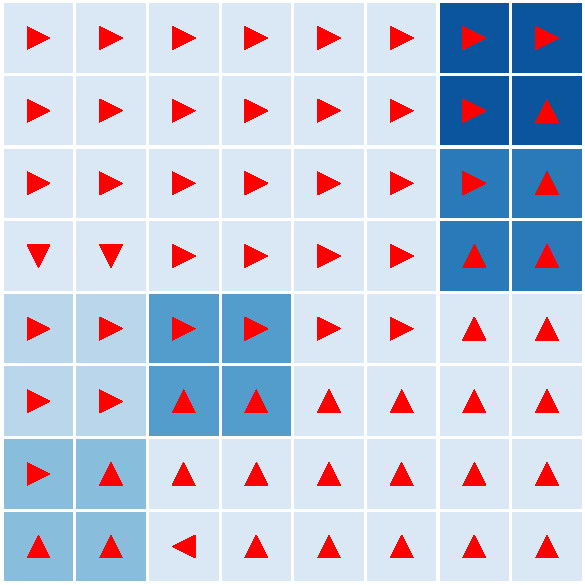
\includegraphics[width=0.13\textwidth]{images/gridworld/macro_cells/grid_8_macro_2/reward_map/true_reward_trim.pdf}}&
%     \MSHangBox{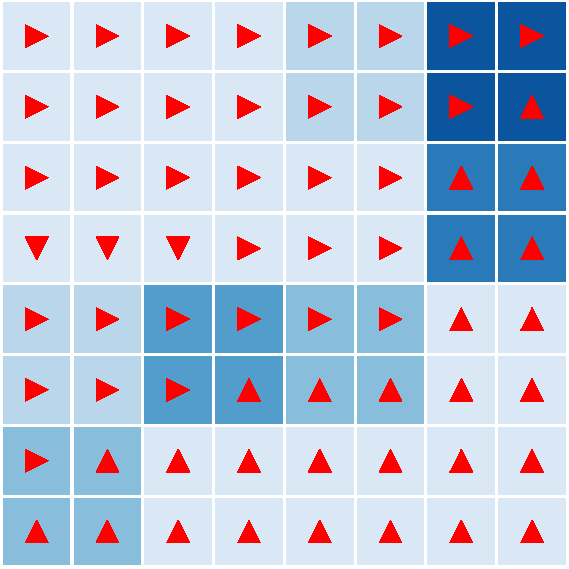
\includegraphics[width=0.13\textwidth]{images/gridworld/macro_cells/grid_8_macro_2/reward_map/maxent_reward_trim.pdf}}&
%     \MSHangBox{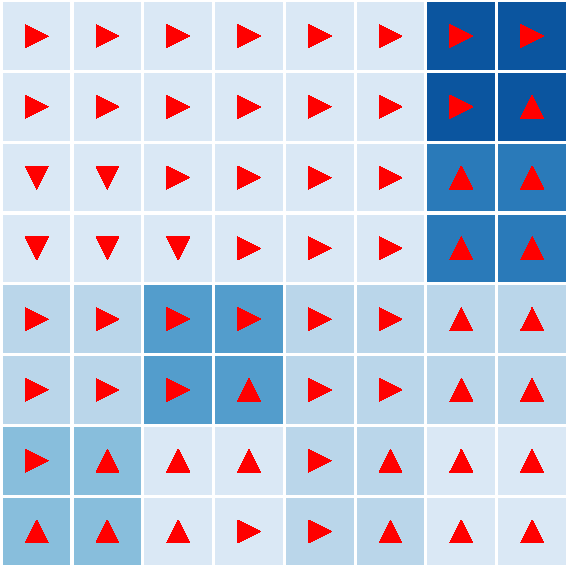
\includegraphics[width=0.13\textwidth]{images/gridworld/macro_cells/grid_8_macro_2/reward_map/ccp_reward_2_trim.pdf}} \\
%     True Reward & MaxEnt & CCP \\
%     \end{tabular}
%     \caption{ Reward distribution for macro cells with gridsize 8 and macro cell size 2 using 10 trajectories. Dark - high reward, Light - low reward. }
%     \label{fig:img_reward_map_gridworld_macro_cell}
% \end{figure}

% \begin{figure}[t]
% \centering
%   \begin{tabular}{c}
%     \MSHangBox{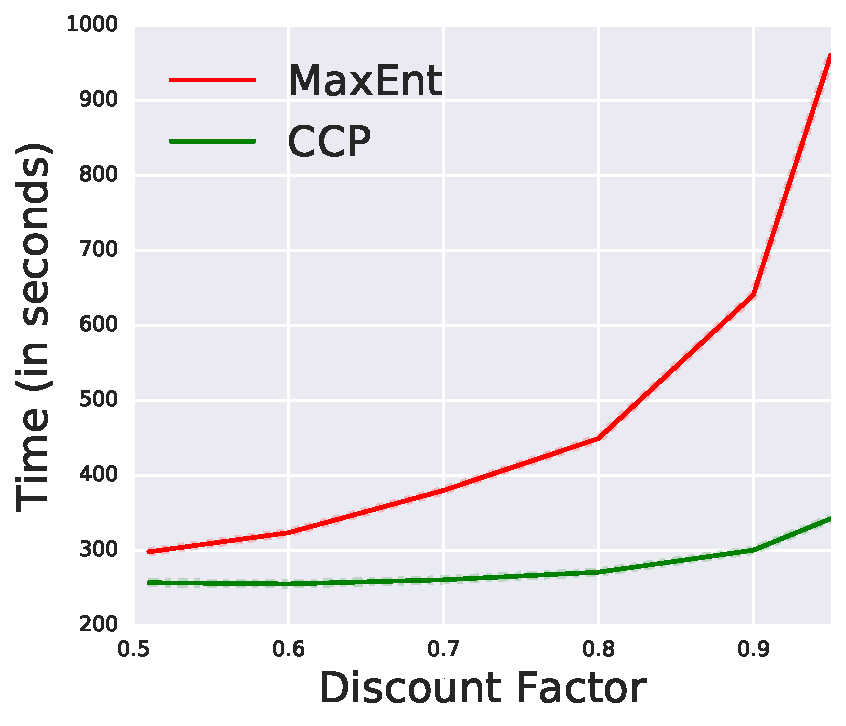
\includegraphics[width=0.4\textwidth]{images/gridworld/fixed_target_wind_30/timeit_maxent_vs_ccp_grid_32_per_discount.pdf}}
%   \end{tabular}
%     \caption{Computation time (in seconds and averaged over multiple runs) comparison between MaxEnt and CCP for Gridworld with gridsize of 32. Each experiment was run for 50 iterations. }
%     \label{fig:img_gridworld_maxent_vs_ccp_time_discount}
% \end{figure}

Similar to previous works \cite{abbeel2004apprenticeship, klein2012inverse}, we use a car driving simulator in a linear reward setting. The goal in this environment is to drive on a multi-lane highway without crashing. The agent's car can either move left or right, accelerate, decelerate or keep a constant speed. We use a hand tuned reward, which penalizes off-road driving and collisions while favoring high speed. 

For our reward feature vector, we use a discretization of the state space. In the simplest case, similar to, Klein \emph{et al.} \yrcite{klein2012inverse}, we parameterize the state space using 9 horizontal positions for the user's car, 3 horizontal and 9 vertical positions for the closest traffic's car and 3 speeds. This gives us a feature vector of size $\mathcal{R}^{729}$. To scale this representation to larger MDPs, we increase each of the above MDP parameters, such as, car speed, number of lanes \emph{etc.}. However, a one-hot feature representation, as used in Klein \emph{et al.} does not scale to such large MDPs. Hence for large MDPs, we group adjacent lanes and closest traffic car's position together, to keep the feature vector representation compact.

\begin{figure}[t]
\centering
  \begin{tabular}{cc}
    \MSHangBox{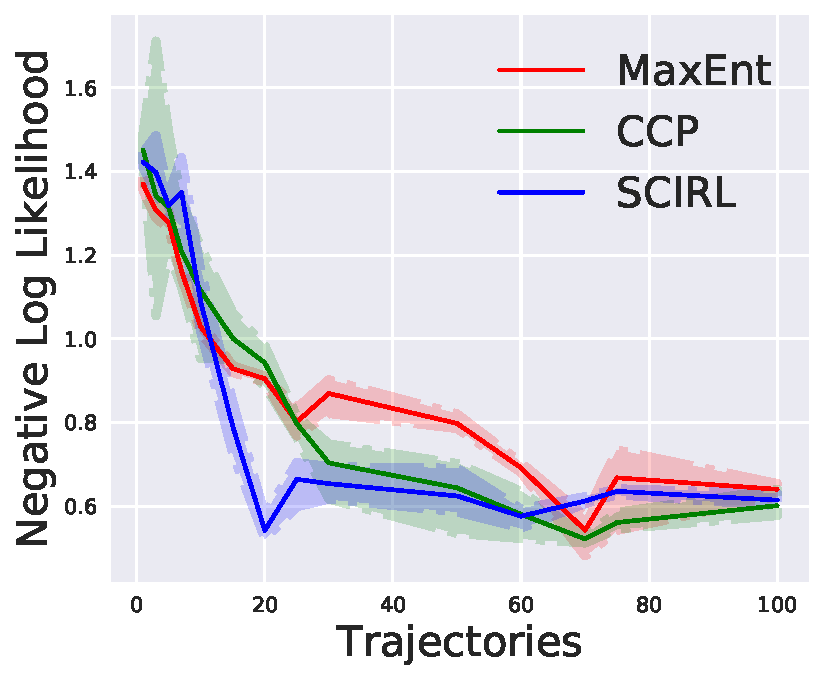
\includegraphics[width=0.22\textwidth]{images/highway/medium_mdp/test_nll.pdf}}&
    \MSHangBox{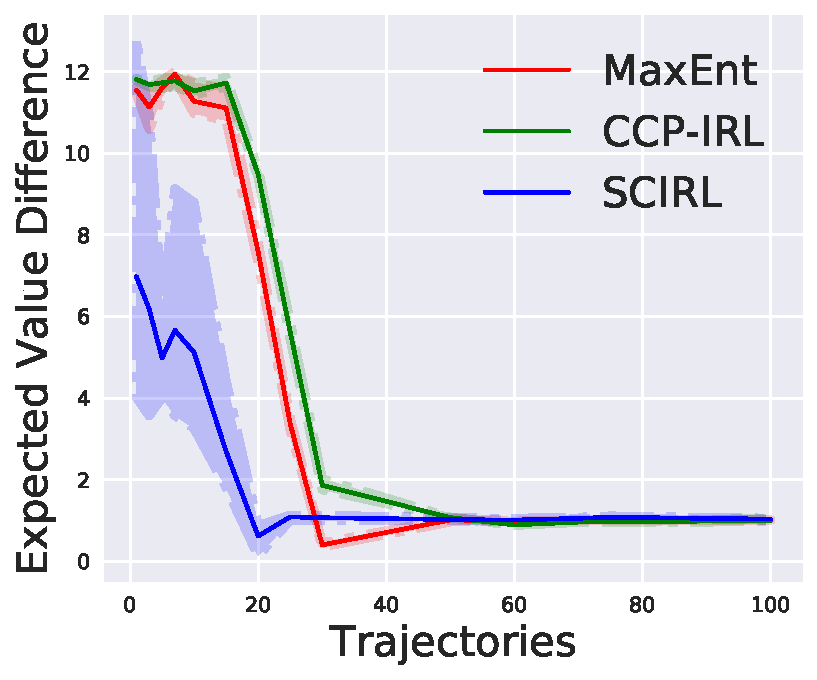
\includegraphics[width=0.22\textwidth]{images/highway/medium_mdp/test_evd.pdf}}
    \end{tabular}
    \caption{Results for Highway MDP with 5,000 states. Left: Minimum NLL results with varying number of trajectories. Right: Expected Value Difference results. As seen the sample complexity of CCP-IRL is very close to SCIRL and not much worse than MaxEnt-IRL.}
    \label{fig:img_maxent_vs_ccp_gridworld_macro_cell}
\end{figure}

First, we analyze the performance of CCP-IRL given different amounts of expert trajectories.
Figure \ref{fig:img_maxent_vs_ccp_gridworld_macro_cell} compares the NLL and EVD results against increasing number of expert trajectories.
As seen above, all algorithms show poor performance given very few trajectories (< 20 trajectories).
However, with moderate number of trajectories ($\sim$30) all algorithms approach expert behavior, although, CCP-IRL requires slightly more number of trajectories as compared to MaxEnt-IRL. This is expected given that CCP-IRL requires consistent CCP estimates to match expert behavior. However, interestingly, SCIRL requires less data compared to both MaxEnt-IRL and CCP-IRL. We believe one reason for this is that SCIRL is solving a max-margin problem to directly imitate the expert, this can often be easier for simple MDPs. 

We also verify the computational advantage for CCP-IRL across large state spaces ($|S| \in \{10^3, 10^6\}$) in Table~\ref{table:table_results_macro_cells}. CCP-IRL is almost 10$\times$ faster than MaxEnt-IRL, across both large and small state spaces. This gives a huge advantage when running on large spaces since MaxEnt-IRL is prohibitively expensive in such settings. Also, since SCIRL follows a completely different algorithmic approach to IRL, we do not directly compare the computation time for SCIRL with entropy based IRL approaches. However, we do note that in preliminary experiments we found SCIRL to be at least $2\times$ as fast as CCP-IRL.
%However, SCIRL is much faster than both CCP-IRL and MaxEnt-IRL. This is because rather than solving a complex maximum entropy problem, SCIRL solves a multi-class classification problem using the max-margin approach. Although, SCIRL is able to infer the appropriate reward in our setting, such structured margin classifiers suffer from other drawbacks as discussed in \cite{ziebart2010modeling}. Additionally, as we show below, SCIRL works for linear reward parameterization only, which greatly reduces its applicability in complex scenarios. Despite this, the efficacy of the SCIRL and CCP-IRL reflect that, combining CCP estimates from expert trajectories with the MDP structure can significantly boost IRL performance without sacrificing the sample complexity too much. 

\subsection{Objectworld: Evaluating Non-Linear Rewards}

We now look at CCP-IRL's performance when the true reward function is a non-linear parameterization of the feature vector.
For this, we use the Objectworld \cite{levine2011nonlinear} environment since the reward function is a non-linear function of state features.
Similar to related work \cite{wulfmeier2015maximum}, we use a Deep Neural Network (DNN) as the non-linear function approximator.
As before, we verify both (1) the computational advantage provided by CCP-IRL (DeepCCP-IRL) and (2) the data requirement for CCP-IRL in the above scenario.

The Objectworld environment consists of a grid of $N \times N$ states. At each state the agent can take 5 actions, including movement in 4 directions and staying in place. Spread through the grid are random objects, each with an inner and outer color. Each of these colors is chosen from a set of $C$ colors. The reward for each cell(state) is positive if the cell is within distance 3 of color 1 and distance 2 of color 2, negative if only within distance 3 of color 1 and zero in all other cases. For our feature vector we use a continuous set of values $x \in \mathbb{R}^{2C}$, where $x_i$ and $x_{i+1}$ is the shortest distance from the state to the \emph{i'th} inner and outer color respectively. Since the reward is only dependent on two colors, features for other colors act as distractors. However, since SCIRL requires linear parameters we expand the features to include polynomial basis for SCIRL only. We would like to note that although such an approach can be used to approximate non-linear rewards, it requires significant hand-tuning and is not generalizable to more complex reward scenarios. 

\begin{table}[t]
\centering
\def\arraystretch{1.2}% 
\begin{tabular}{|c|c|c|c|}
\hline
Experiment Setting & MaxEnt & CCP & Speedup \\\hline

%Grid size: 16, C = 2 & 1622.63 & \textbf{296.43} & $\mathbf{5}\times$ \\
Grid size: 32, C = 2 & 9115.50 & \textbf{1580.22} & $\mathbf{6}\times$ \\
%Grid size: 16, C = 8 & 2535.38  & \textbf{545.95} & $\mathbf{5}\times$ \\
Grid size: 32, C = 8 & 19445.66 & \textbf{4799.02} & $\mathbf{4}\times$ \\
Grid size: 64, C = 4 & 27661.66 & \textbf{4634.14} & $\mathbf{6}\times$ \\
Grid size: 128, C = 4 & 237278.48 & \textbf{27886.87} & $\mathbf{8}\times$ \\
\hline
\end{tabular}
\caption{Computation time (in seconds and averaged over multiple runs) comparison between MaxEnt and CCP for Objectworld. Each experiment was run for the same number of iterations with similar settings. }
\label{table:table_results_objectworld}
\end{table}

\begin{figure}[t]
\centering
  \begin{tabular}{cc}
    \MSHangBox{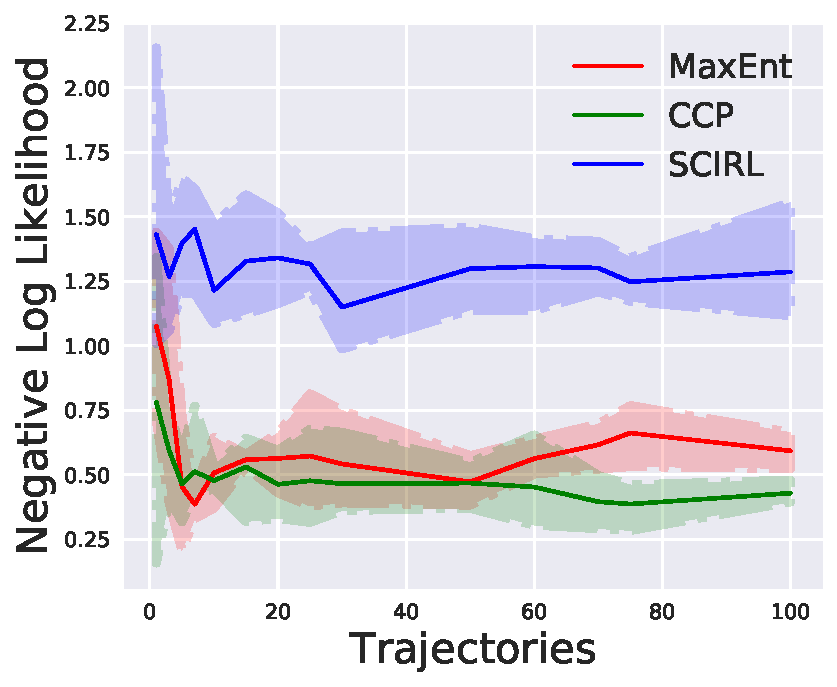
\includegraphics[width=0.23\textwidth]{images/objectworld/grid_32_obj_30_algo_3/test_nll_algo_3.pdf}}
    \MSHangBox{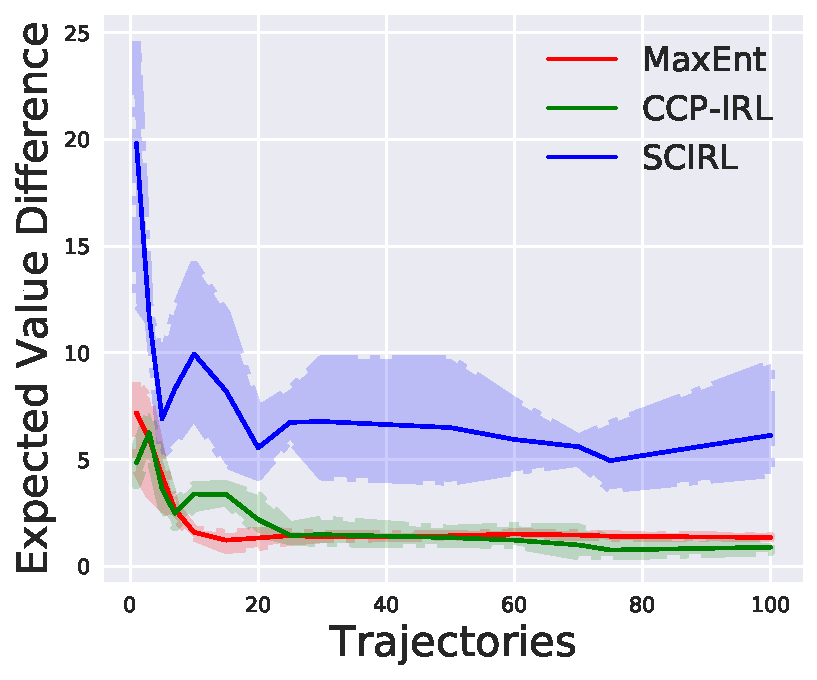
\includegraphics[width=0.23\textwidth]{images/objectworld/grid_32_obj_30_algo_3/test_evd_algo_3.pdf}}
  \end{tabular}
    \caption{Results on ObjectWorld with gridsize of 32 and 2 colors. Left: NLL results on test trajectories. Right: Expected Value Difference results. }
    \label{fig:img_objectworld_maxent_vs_ccp_lr_01}
\end{figure}

\begin{figure}[t]
\centering
  \begin{tabular}{cc}
    \MSHangBox{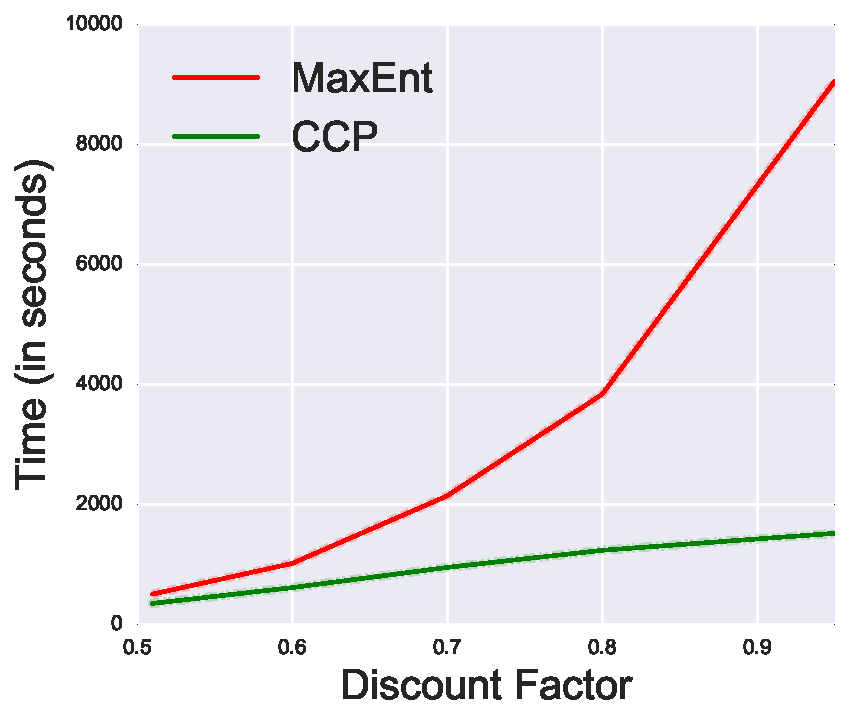
\includegraphics[width=0.23\textwidth]{images/objectworld/timeit_maxent_vs_ccp_grid_32_discount_value.pdf}}
    \MSHangBox{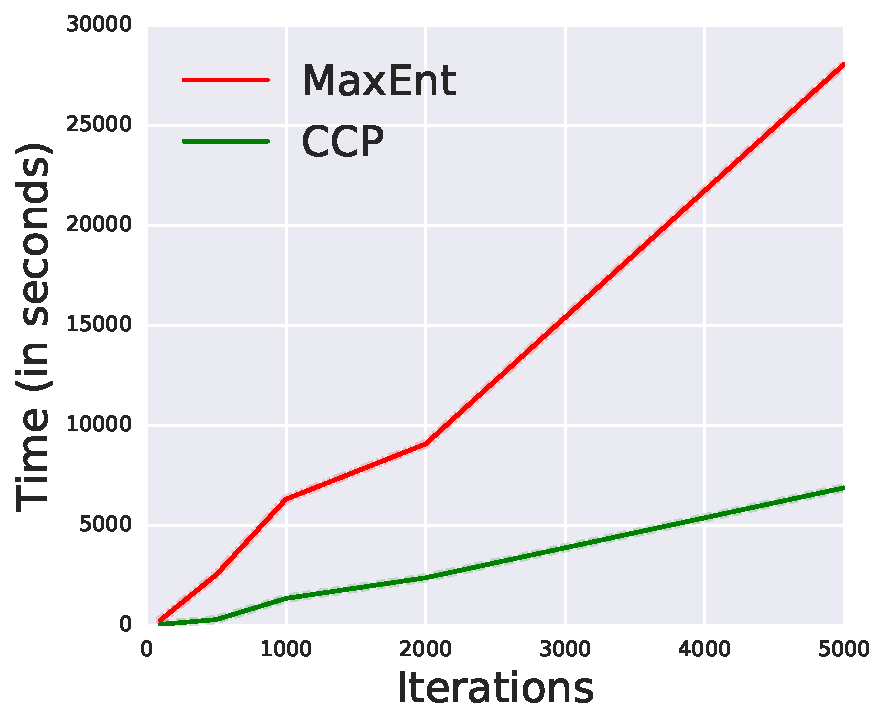
\includegraphics[width=0.23\textwidth]{images/objectworld/timeit_maxent_vs_ccp_grid_16_per_iter.pdf}}
  \end{tabular}
    \caption{Left: Time variance between MaxEnt-IRL and CCP-IRL with increasing discount values. Right: Time variance between MaxEnt-IRL and CCP-IRL with increasing number of iterations. As expected CCP-IRL shows little computation increase with more complex MDPs.}
    \label{fig:img_objectworld_maxent_vs_ccp_time_results}
\end{figure}

\begin{figure}[t]
\centering
  \begin{tabular}{ccc}
    \MSHangBox{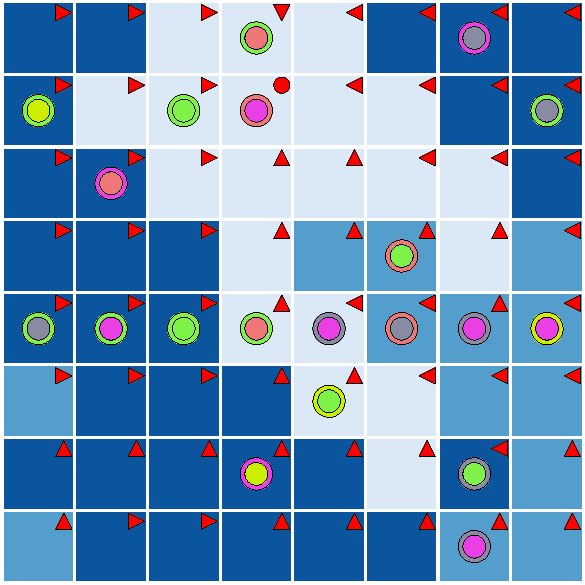
\includegraphics[width=0.13\textwidth]{images/objectworld/grid_8_object_20_color_5/reward_map/true_reward_trim.pdf}}&
    \MSHangBox{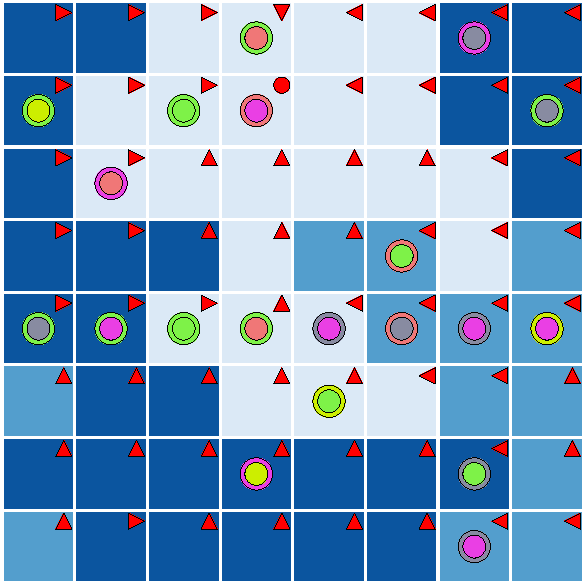
\includegraphics[width=0.13\textwidth]{images/objectworld/grid_8_object_20_color_5/reward_map/maxent_reward_trim.pdf}}&
    \MSHangBox{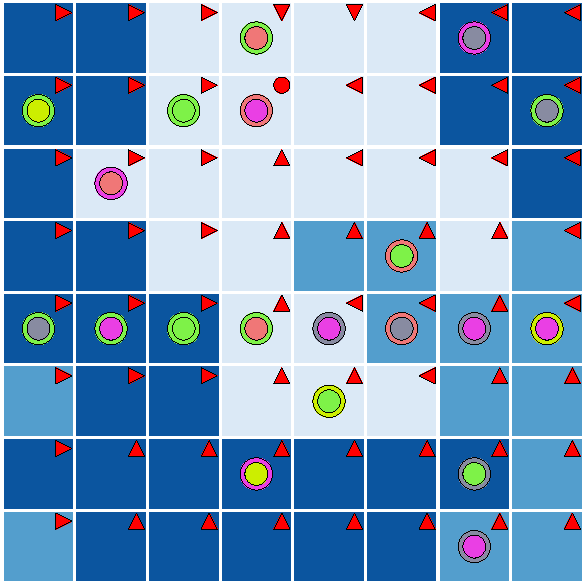
\includegraphics[width=0.13\textwidth]{images/objectworld/grid_8_object_20_color_5/reward_map/ccp_reward_trim.pdf}} \\
    True Reward & MaxEnt & CCP \\
    \end{tabular}
    \caption{ Reward distribution for Objectworld with gridsize 8 using 30 trajectories and 5 colors. Dark - low reward, Light - high reward. We also plot the inner and outer color of each object. \textit{Pink} - color 1 \textit{Orange} - color 2, other colors are distractors. \textit{Figure best viewed in electronic version.} }
    \label{fig:img_reward_map_objectworld}
\end{figure}

We use similar deep neural network architecture for both CCP-IRL and MaxEnt-IRL. Precisely, we use a 2-layer feed-forward network with rectified linear units. We use the Adam \cite{kingma2014adam} optimizer with the initial learning rate set to $10^{-3}$.

We quantitatively analyze the performance of our proposed DeepCCP-IRL algorithm in Figure \ref{fig:img_objectworld_maxent_vs_ccp_lr_01}, which compares the NLL and EVD results. Notice that as observed before, with few expert trajectories all algorithms perform poorly. However, both DeepMaxEnt-IRL and DeepCCP-IRL match expert performance with moderate number of trajectories ($\approx 20$). Although, as seen before comparatively CCP-IRL requires few more trajectories as compared to MaxEnt-IRL, to get consistent CCP estimates. In contrast, SCIRL approach fails to learn the appropriate parameters in this setting. Although, given more expressive non-linear features a linear parameterization could suffice for this simple problem, it is not clear how SCIRL can be generally extended to non-linear reward parameters. 
%In contrast, the CCP-IRL approach easily generalizes to non-linear settings with a small increase in the sample complexity.

% Also, we qualitatively look at the inferred reward to verify how well the DNN is able to approximate the non-linear reward. Figure \ref{fig:img_reward_map_objectworld} plots the inferred rewards against the true reward function. Notice that both algorithms capture the non-linearities in the underlying reward function and consequently match the expert behavior. Thus, a deep neural network suffices as a non-linear function approximator for CCP-IRL.

We now analyze the computation gain in the non-linear case. Table \ref{table:table_results_objectworld} shows the computation time for different sized state spaces and different sized feature vectors. Notice that DeepCCP-IRL is more than 5$\times$ as fast as DeepMaxEnt-IRL across small and large state spaces. Thus, we see that CCP-IRL provides a large computation advantage for the non-linear case as well. Further, we also note that for more complex MDP problems the computational advantage for CCP-IRL would be much larger, since CCP-IRL only runs the MDP step once. To illustrate this, we run the Objectworld experiment with different discount values and different number of iterations respectively, since lower discount value and fewer iteration imply an easier MDP problem to solve. Figure \ref{fig:img_objectworld_maxent_vs_ccp_time_results} shows the computation time for DeepCCP-IRL and DeepMaxEnt-IRL in both these settings. As can be seen, as the MDP problem becomes more complex, MaxEnt-IRL's computation time increases almost exponentially while CCP-IRL approach scales sub-linearly.

Thus, the efficacy of CCP-IRL reflects that, combining CCP estimates from expert trajectories with the MDP structure can help significantly boost IRL performance without sacrificing the sample complexity too much. Although, the sample complexity for CCP-IRL is greater than MaxEnt-IRL, we note that a full fledged sample complexity analysis between them is beyond the scope of our initial work.

%%%%%%%%%%%%%%%%%%%%%%%%%%%%%%%%%%%%%%%%%%%%%%%%%


\section{Related Work \& Discussion}

Past work in scaling IRL for large spaces has looked at discrete and continuous spaces separately. Applying Max-Ent IRL to continuous spaces is more challenging. Trivially, we could discretize the continuous space and then apply MaxEnt-IRL algorithm directly. However, this scales exponentially with respect to the state space and is thus infeasible in practice. 
Hence, more sophisticated algorithms are required to extend MaxEnt-IRL to continuous spaces.

For discrete spaces, past work such as, \cite{huang2015approximate} has mainly focused on approximating the value iteration step in IRL. However, since the MDP problem is still being solved at every step of an iterative procedure this does not scale to very large spaces. For continuous domains, most algorithms use local approximation to estimate the partition function in MaxEnt-IRL. Using local approximations requires giving up on global optimality, but allows the algorithms to scale to high dimensional continuous domains \cite{levine2012continuous, kalakrishnan2013learning, finn2016guided}.

Alternately, some IRL algorithms have focused on a smaller subset of MDP problems. Todorov \yrcite{todorov2007linearly} introduced a new class of MDPs which are linearly solvable. Dvijotham and Todorov \yrcite{dvijotham2010inverse} present an efficient IRL algorithm, which they call OptV, for these MDPs. However, this new class of MDP's only solve a restricted form of general MDP formulation and is thus not applicable in all scenarios. 
Also, since OptV finds the parameters in value-function space it is not clear how meaningfully these features can be transferred across different tasks \cite{levine2012continuous}.
%In contrast, our work makes no such approximation of the general MDP framework and is thus applicable everywhere.

Although not directly related to entropy based IRL approaches, but similar in spirit to our work, is SCIRL \cite{klein2012inverse}. SCIRL assumes linear reward parameters and uses the feature expectation of the expert in a multi-class classification framework. SCIRL uses a max-margin planning algorithm for their classification framework. However, SCIRL is very different from CCP-IRL, since a classification framework has no notion of the MDP problem being solved and tries to directly imitate the expert behavior. For more discussion on the differences between IRL and max-margin planning approach we refer the reader to \cite{Ratliff2006, ziebart2010modeling}. Another key restriction of their work is that the reward must be expressed as a \textit{linear combination} of features only.\footnote{\cite{klein2012inverse} suggest using basis functions to generate flexibility, however, this introduces another layer of approximation.}

% The key restriction in that paper is that the reward function must be expressed as a linear combination of basis functions of states. A key advantage of CCP-IRL is the ability to estimate reward functions semi-parametrically, a result due to \cite{magnac} which we discuss in the appendix. In addition, CCP-IRL allows us to leverage properties of finite-dependence to further reduce computational burden in more general environments. These results are discussed in \cite{arcidiacono2014nonstationary}.

In contrast to previous work, our CCP-IRL algorithm is generally applicable, as it makes no assumption on the MDP framework, and is applicable to both linear and non-linear reward parameterizations. Additionally, the CCP approach can also be used to estimate the reward in a completely \textit{non-parametric} setting as well, a result due to \cite{magnac}, which we discuss in the Appendix.
%Also, the optimizations used to scale MaxEnt-IRL to continuous spaces are orthogonal to CCP-IRL. Thus, it would be interesting to see how the CCP-IRL framework can be extended to these settings.
In this work we focus on discrete problem settings to introduce the key insights from CCPs in a well understood paradigm. Although CCPs are applicable to situations with continuous state or action spaces \cite{altuug1998effect}. There has also been progress in applying CCP-like estimators to single dimensional continuous controls in complex environments, such as dynamic strategic settings. \cite{pesendorfer} uses a two-step approach to estimate rewards in a dynamic pricing game. It is not yet clear how CCPs extend to high-dimensional continuous control tasks in robotics. We leave this for future work.

In conclusion, CCP-is more generalizable than other related frameworks. Below, we discuss some of the other extensions relevant in AI research while also discussing one specific instance of this extension in the Appendix.

%%%%%%%%%%%%%%%%%%%%%%%%%%%%%%%
%%%%%%%%%%%%%%%%%%%%%%%%%%%%%%%

\textbf{Discussion:} 
% CCP framework helps in the unidentification of the reward formulation
% CCP formulation helps in using other empirial models developed by economists e.g. what if we use a different form of human optimality.
We now discuss some extensions of the CCP framework as used in economics which are relevant in robotics and AI research.  
The CCP framework provides methods to investigate the well known under-identification problem in IRL. Some recent work \cite{amin2017repeated} has focused on the unidentifiability problem in IRL. In \cite{amin2017repeated} the authors focus on identification guarantees when the agent can choose the task rewards in multiple fixed environment settings. In contrast, the CCP approach can be used to clarify necessary assumptions to ensure a ``unique" mapping from trajectories to the reward functions \cite{magnac}. 

The CCP approach is also used successfully in multi-agent settings where strategic situations generally lead to multiple equilibria. Any IRL algorithm that \emph{solves} the DP numerically will require an ad-hoc equilibrium selection rule. Moreover, there is no data-driven way to ensure the selection rule is identifying the equilibrium in the data. It is therefore highly likely that an IRL algorithm can match the data by selecting the wrong reward parameters and the wrong equilibrium. In other words, matching the data is not enough to guarantee the accuracy of measurements. However, with CCPs and a dataset on a single path of play, it is possible to estimate rewards consistently. The data allow us to directly estimate the policy functions of the equilibrium in the data. The CCP representations of the value function therefore are for the correct equilibrium. It is then possible to correctly estimate the reward function, without having to solve the game and to correctly select the equilibrium in the data \cite{pese}.

Furthermore, the CCP framework opens up the possibility of estimating rewards in non-stationary environments. The CCP framework leads computational simplifications in settings where actions terminate the decision problem or a sequence of actions ``reset" the future state distributions \cite{arcidiacono2014nonstationary}. These results allow us to represent future values as arbitrary sequences of future CCPs.
% But to highlight the connections between IRL and CCP estimation, in this paper we focus only on stationary discrete choice optimization problems,

%Finally, we look at the data requirement for CCP-IRL. A complete theoretical analysis of sample complexity of CCPs is beyond the scope of our initial work. However, we would like to refer the reader to Aguirregabiria and Mira \yrcite{aguirregabiria2002swapping} which discuss some sample properties of CCP estimators. More importantly, the authors show that one-step CCP estimators (such as CCP-IRL) can have large bias with insufficient data.  To reduce this bias they introduce a successive iteration procedure which results in a sequence of estimators. They further show that this iteration until convergence will realize the original MaxEnt-IRL estimator.

Finally, from the robotics perspective, the process of learning the CCPs is exactly Behavior Clongin (BC), where the policy is learned directly from demonstrations without making the reward function explicit. The CCP-IRL framework can then be interpreted as, an behavior cloning phase followed by a inverse reinforcement learning phase that makes use of a fully specified policy to estimate the reward function.

\section{Conclusion}

% Edit later... place holder

We have described an alternative framework for inverse reinforcement learning (IRL) problems that avoids value function iteration or backward induction. In IRL problems, the aim is to estimate the reward function from observed trajectories of a Markov decision process (MDP). We first analyze the decision problem and introduce an alternative representation of value functions due to \cite{hotz}. These representations allow us to express value functions in terms of empirically estimable objects from action-state data and the unknown parameters of the reward function. We then show that it is possible to estimate reward functions with few parametric restrictions. 

%%%%%%%%%%%%%%%%%%%%%%%%%%%%%%%%%%%%%%%%%%


\bibliography{references}
\bibliographystyle{icml2018}




% \clearpage
% \section*{Appendix for "Conditional Choice Probability Inverse Optimal Control"}


% \section{Identification Of Reward Functions}
% In econometrics, ``identification" refers to the process of determining whether observed distributions in the data can be mapped into a unique set of parameters of a model. Identification assumes the investigator has access to an infinitely large data set and is not constrained by estimation error. The question in this setting is whether it is mathematically possible to construct a unique mapping from data to the parameters of interest. In the MDP setting, we can determine whether data on states and actions is sufficient to identify the reward function and to what extent parametric assumptions are required. \cite{pese} prove that the solution to a MDP can be represented as an equation system that is linear in the reward function (See Lemma 1 in that paper). Identification then reduces to determining whether a linear equation system has a unique solution. In particular, \cite{pese} provide conditions for identification in multi-agent settings, which are very similar to single-agent decision problems.

% We present one type of identification argument following \cite{bajari} where we assume that one action has a zero payoff in every state. 
% We will now show how the value function is related to the CCPs by introducing the choice-specific value function. Denote the choice-specific value function as the value associated with action $a$ excluding $\epsilon_a$ as:
% \begin{align}
% V_a(x_t) &\triangleq r(a,x_t)+\beta \sum_{x_{t+1}\in\mathcal{X}}T(x_{t+1}|x_t,a) \overline{V}(x_{t+1}) \\
% &=r(a,x_t)+\beta \sum_{x_{t+1}\in\mathcal{X}}T(x_{t+1}|x_t,a) E_{\vec{\epsilon}_{t+1}}
% \max_{a'}\left\{V_{a'}(x_{t+1})+\epsilon_{t+1})\right\}\label{eq:vamax_id}
% \end{align}
% Define the value function difference for action $a$ and $a_0$ as:
% \begin{align}
% \Delta_a(x)\triangleq V_a(x)-W_{a_0}(x).
% \end{align}
% The base action $a_0$ is selected, one action for each state, for which the immediate reward is normalized to zero. Now add and subtract $W_{a_0}(x_{t+1})$ within the max operator in (\ref{eq:vamax}), introduce the short-hand $T^{x_{t+1}}_{x_t,a}$, and expanding the expectation with TIEV yields:
% \begin{eqnarray}\label{eq:cond_choice_v}
% V_a(x_t)=r(a,x_t)+\beta \sum_{x_{t+1}} T^{x_{t+1}}_{x_t,a}  \\ 
% \left[W_{a_0}(x_{t+1})+\ln\left[1+ \sum_{a'\neq a_0}\exp(\Delta_{a'}(x_{t+1}))\right]+\gamma\right]\label{eq:vax}
% \end{eqnarray}
% We now have the choice-specific value function defined in terms of the value function difference $\Delta_{a}$.



% \subsection{Connecting Choice-Specific Value Function to CCPs}

% We will now proceed to expand the residual in terms of a ratio of CCPs. Recalling the definition of CCPs and choice-specific value function from Equations (\ref{eq:ccps}) and (\ref{eq:vax}):
% \begin{eqnarray}
% \sigma(a|x_t)=\frac{\exp\left(V_a(x_t)\right)}{\sum_{a'} \exp\left(V_{a'}(x_t)\right)}.
% \end{eqnarray}


% Multiplying and dividing by $\exp(-W_{a_0}(x_t))$ leads to
% \begin{eqnarray}
% \sigma(a|x_t)=\frac{\exp(V_a(x_t)-W_{a_0}(x_t))}{\sum_{a'} \exp(V_{a'}(x_t)-W_{a_0}(x_t))}=\frac{\exp(\Delta_a(x_t))}{\sum_{a'} \exp(\Delta_{a'}(x_t))}.
% \end{eqnarray}


% It is clear from the above that value function differences between action $a$ and $a'$ are equal to:
% \begin{eqnarray}
% \frac{\sigma(a'|x_t)}{\sigma(a_0|x_t)}=
% \left[
% \frac
%   {\exp(\Delta_{a'}(x_t))}
%   {\sum_{a''} \exp(\Delta_{a''}(x_t))}
% \right]
% \left[\frac{1}{\sum_{a''} \exp(\Delta_{a''}(x_t))}\right]^{-1}=\exp(\Delta_{a'}(x_t))
% \end{eqnarray}
% %
% %
% %
% Using the CCP ratio, the value function for the base action $a_0$ can be expressed as:
% \begin{eqnarray}
% W_{a_0}(x_t) 
% = 
% \beta\sum_{x_{t+1}}
% T(x_{t+1}|x_t,a_0) 
% \left[W_{a_0}(x_{t+1})+\ln\left[1+ \sum_{a'\neq a_0}\frac{\sigma(a'|x_{t+1})}{\sigma(a_0|x_{t+1})}\right]+\gamma\right]
% \end{eqnarray}\label{eq:va0}

% \subsection{Solving for the Optimal Value Function}

% Since we have expressed the choice-specific (a base action) value function in terms of just the transition function and CCPs, we can now estimate $W_{a_0}$ as a fixed point of the above linear equation -- without the knowledge of the full value function or the reward function. In particular, stacking the value function  $W_{a_0}$ for all states yields a $m_x\times 1$ vector:
% \begin{eqnarray}
% \mathbf{V}_0\equiv \left[\begin{array}{c} W_{a_0}(x_1)\\W_{a_0}(x_2)\\\vdots\\ W_{a_0}(x_{m_x})\end{array}\right]
% \end{eqnarray}
% and $\mathbf{T}$ is the transition matrix with entry $T(x_{j}|x_m,a_0)$ for the $m$th row and the $j$th column. 

% Also define the $m_x\times 1$ vector $\mathbf{\Gamma}$ as:
% \begin{align}
% \mathbf{\Gamma} \equiv \left[\begin{array}{c} 
% \ln(1+\sum_{a'\neq a_0}\sigma(a'|x_1)/\sigma(a_0|x_1))\\
% \vdots\\
% \ln(1+\sum_{a'\neq a_0}\sigma(a'|x_{m_x})/\sigma(a_0|x_{m_x}))\\
% \end{array}\right].
% \end{align}

% Then we can write system of equations in matrix form as:
% \begin{align}
% \mathbf{V}_0 = \beta \mathbf{T} [\mathbf{V}_0 + \mathbf{\Gamma}]
% \label{eq:v0_fp}
% \end{align}
% which leads to
% \begin{align}
% \mathbf{V}_0 = [I-\beta \mathbf{T}]^{-1}\beta \mathbf{T} \mathbf{\Gamma}.
% \label{eq:v0_inv}
% \end{align}

% The above is the unique fixed point. The value function for every state can then be estimated as:
% \begin{eqnarray}
% V_a(x_t)=\ln(\sigma(a|x_t))-\ln(\sigma(a_0|x_t))+W_{a_0}(x_t).\label{eq:v_backout}
% \end{eqnarray}



% \subsection{Backing Out the Reward Function}

% We can go further to estimate the reward values $r(a, x_t)$ for $a$ and every state $x_t$ without the need for a costly gradient descent algorithm. We can do this by simply backing out the reward values using equation \ref{eq:va}:
% \begin{align}\label{eq:reward}
% r(a,x_t)
% =V_a(x_t)- \nonumber\\ \beta\sum_{x_{t+1}\in\mathcal{X}}T(x_{t+1}|x_t,a) 
% \left\{
% W_{a_0}(x_{t+1})
% +\ln
%  \left(
%     1 + \sum_{a'\in\mathcal{A}}\frac{\sigma(a|x_{t+1})}{\sigma(a_0|x_{t+1})}
%   \right)
% \right\}.
% \end{align}


% \newpage
% Return to ex-ante

% \begin{align} \label{eq:exantebellman}
% \begin{split}
% \overline{V}(x_t) & = E_{\vec{\epsilon}_t}\Big[\max_{a\in\mathcal{A}} \big\{r(x_t,a)+\epsilon_{at} \\
% & +\beta  \cdot E_{x_{t+1}|a,x_t} \left[ \overline{V}(x_{t+1}) \right] \big\}\Big]\\
% &=\sum_{a\in\mathcal{A}} \sigma(a|x_t) \left[r(x_t,a)+\tilde{\epsilon}(a|x_t)+\beta \sum_{x_{t+1}\in\mathcal{X}} T(x_{t+1}|x_t,a) \overline{V}(x_{t+1})\right]
% \end{split}
% \end{align}
% where 
% \[
% \tilde{\epsilon}(a|x_t)
% \]
% is the expected value of epsilon conditional on $a$ being optimal at state $x_t$. We know from Hotz Miller that this is equal to $\gamma-\ln\sigma(a|x_t)$ and is therefore only a function of the CCPs. Now stack the ex-ante value function over all states:
% \begin{align}
%     \begin{split}
%     \overline{V}=\sum_{a}S(a) *\left[ R(a)+\tilde{\epsilon}(a)+\beta T(a) \overline{V}\right]
%     \end{split}
% \end{align}
% where:
% \[
% \overline{V}=\left[\begin{array}{c}\overline{V}(x_1)\\\vdots\\\overline{V}(x_{|\mathcal{X}|}\end{array}\right]
% \]
% \[
% R(a)=\left[\begin{array}{c}r(x_1,a)\\\vdots\\ r(x_{|\mathcal{X}|},a)\end{array}\right]
% \]
% \[
% T(a)=\left[\begin{array}{ccc}
% T(x_1|x_1,a),\dots,T(x_{|\mathcal{X}|},x_1,a)\\
% \vdots\\
% T(x_1|x_{|\mathcal{X}|},a),\dots,T(x_{|\mathcal{X}|},x_{|\mathcal{X}|},a)\\
% \end{array}\right]
% \]
% \[
% S(a)=\left[\begin{array}{c}\sigma(a|x_1)\\ \vdots\\ \sigma(a|x_{|\mathcal{X}|})\end{array} \right]
% \]
% \[
% \tilde{\epsilon}(a)=\left[\begin{array}{c}\tilde{\epsilon}(a|x_1)\\ \vdots \\ \tilde{\epsilon}(a|x_{|\mathcal{X}|})\end{array}\right]
% \]
% Re-arranging :
% \begin{align}
%     \begin{split}
%     \overline{V}-\sum_{a}S(a) *\left[ \beta T(a) \overline{V}\right]=\sum_{a}S(a) *\left[ R(a)+\tilde{\epsilon}(a)\right]
%     \end{split}
% \end{align}
% which we can solve for $\overline{V}$
% \begin{align}
%     \begin{split}
%     \overline{V}=\left[I-\sum_{a}(S(a) \lambda) *\left[ \beta T(a)  \right]\right]^{-1}\left[\sum_{a}S(a) *\left[ R(a)+\tilde{\epsilon}(a)\right]\right]
%     \end{split}
% \end{align}
% where $\lambda$ is a $1\times|\mathcal{X}|$ vector of ones.

\clearpage

% \subsection{Hotz-Miller's CCP Method}

% Our aim in Inverse Reinforcement Learning is to find the parameterized reward function $r(\theta)$ for the given MDP/R. We will now show how we can leverage the non-parameteric estimates of choice conditional probabilities to efficiently estimate the parameters($\theta$) of the reward function for both linear and non-linear parameterization. 
% Denote the choice-specific value function as the value associated with action $a$ excluding $\epsilon_a$ as:
% \begin{align}\label{eq:vamax}
% \begin{split}
% V_a(x_t) &\triangleq r(a,x_t)+\beta \sum_{x_{t+1}\in\mathcal{X}}T(x_{t+1}|x_t,a) \overline{V}(x_{t+1}) \\
% %&=r(a,x_t)+\beta \sum_{x_{t+1}\in\mathcal{X}}T(x_{t+1}|x_t,a) \\
% %& \qquad \times E_{\vec{\epsilon}_{t+1}} \max_{a'}\left\{V_{a'}(x_{t+1})+\epsilon_{t+1})\right\} \\
% &=r(a, x_t) + \sum_{j=1}^{T-t}\beta^{j}E_{x_{t+j}|a_t,x_t} \\
% & \qquad \big[r(x_{t+j}, a_{t+j})+ E_{\epsilon_{t+j}|a_t, x_t}\left[\epsilon(x_{t+j}, a_{t+j})\right] \big]
% \end{split}
% \end{align}

% \textbf{Linear Parameters:} Many traditional IRL algorithms such as, \cite{abbeel2004apprenticeship} \cite{ziebart} assume that the reward is a linear combination of known features $z$. Assuming this we will now show how we can efficiently estimate $V_a(x_t)$ for different values of $r(\theta)$.

% For linear parameterization we can write $r(a, x_t) = z(a, x_t)^T\theta$, where $z(a, x_t)$ are the set of basis functions (features) known to us.
% Notice from \eqref{eq:vamax}, $V_a(x_t)$ is nothing but the expected and discounted sum of future rewards and shock values respectively. Thus we can split \eqref{eq:vamax} into two parts.
% Define $\tilde{z}(a, x_t)$ and $\tilde{e}(a, x_t)$ as the expected and discounted sum of current and future $z$ values and $\epsilon$ values respectively. Given this we can break \eqref{eq:vamax} into,
% \begin{align}\label{eq:choice_specific_linear_param}
% \begin{split}
% V_a(x_t) & = \tilde{z}(a, x_t)^T \theta + \tilde{e}(a, x_t) \\
% \tilde{z}(a, x_{t}, \theta) & = z(a, x_{t}) + \sum_{j=1}^{T-t}\beta^{j} E_{x_{t+j}|a,x_t} \\
% & \qquad \times \left[ z\left(\pi^{*}\big( x_{t+j}, \epsilon_{t+j}, \theta \right), x_{t+j} \big) \right] \\
% \end{split}
% \end{align}
% where $\pi^{*}(x_{t}, \epsilon_{t}, \theta)$ is the optimal policy. We will now show that both $\tilde{z}$ and $\tilde{e}$ need to be estimated only once.
% To achieve this notice that, we can get consistent estimates of $\pi^{*}(x_t, \epsilon_t, \theta)$ from CCPs, hence we can write \eqref{eq:choice_specific_linear_param} as,
% \begin{align}\label{eq:z_tilde_ccp}
% \begin{split}
%   \tilde{z}(a, x_{t}, \theta) & = z(a, x_t) + \sum_{j=1}^{T-t} \beta^{j} E_{x_{t+j}|a_t=a, x_t} \\
%   & \qquad \left[ \sum_{a_{t+j}} P(a_{t+j}|x_{t+j}) z(a_{t+j}, x_{t+j}) \right] \\
%   \end{split}
% \end{align}
% We can very similarly write the above expression for $\tilde{e}(a, x_t, \theta)$ replacing $z(a, x_t)$ with $E[\epsilon_t(a)|x_t, a]$. For notational convenience we define $e(a, x_t) \equiv E[\epsilon_t(a)|x_t, a]$,
% \begin{align}\label{eq:e_tilde}
% \begin{split}
%   \tilde{e}(a, x_{t}, \theta) & = \sum_{j=1}^{T-t}\beta^{j} E_{x_{t+j}|a,x_t} \\
%   %& \qquad \times \left[ e\left(\pi^{*}\big( x_{t+j}, \epsilon_{t+j}, \theta \right), \epsilon_{t+j} \big) \right] \\
%   %& = \sum_{j=1}^{T-t} \beta^{j} E_{x_{t+j}|a_t=a, x_t} \\
%   & \qquad \left[ \sum_{a_{t+j}} P(a_{t+j}|x_{t+j}) e(a_{t+j}, x_{t+j}) \right] \\
%   \end{split}
% \end{align}

% \cite{hotz} show that $e(a, x_t)$ depends on conditional choice probabilities and distribution of $\epsilon$ only. Further, they prove that the mapping between CCPs and choice specific value function is invertible. Using this inverse mapping and assuming TIEV distribution for $\epsilon$, we get $e(a, x_t) = \gamma - \log P(a|x_t)$.

% Thus, both $\tilde{z}(a, x_t)$ and $\tilde{e}(a, x_t)$ depend on CCP values and transition probabilities only. As a result we can efficiently estimate $V_a(x_t)$ for different values of $\theta$ from \eqref{eq:choice_specific_linear_param} using simple matrix computations. The only real computation involved is in calculating $\tilde{z}(a, x_t)$ and $\tilde{e}(a, x_t)$, both of which need to be done only once. Compare this to \cite{ziebart} where $V_a(x_t)$ needs to be calculated via expensive DP at every $\theta$ value. 
% %These can be estimated by solving the DP problem using backwards recursion from \eqref{eq:z_tilde_ccp} and \eqref{eq:e_tilde} respectively, which is similar to Algorithm 9.1 in \cite{ziebart_phd}.

% We will now show that the above estimation procedure can be simplified into a fixed point iteration algorithm. Let,
% \begin{align}\label{eq:z_tilde_matrix}
% Z(x) = \sum_{a}P(a|x)\tilde{z}(a, x)
% \end{align}
% this allows us to rewrite \eqref{eq:vamax} as,
% \begin{align}\label{eq:z_tilde_from_Z}
% \tilde{z}(a, x) = z(a, x) + \beta\sum_{x'}T(x'|a, x)Z(x')
% \end{align}

% Multiplying the above expression with $P(a|x)$ and summing over all actions we get,
% \begin{align}\label{eq:z_tilde_recursion}
% \begin{split}
% \sum_{a}P(a|x)\tilde{z}(a|x) &= \sum_{a}P(a|x) \\
% & \times \left\{z(a, x) + \beta\sum_{x'}T(x'|a,x)Z(x') \right\}
% \end{split}
% \end{align}

% The LHS above is the definition of $Z(x)$ \eqref{eq:z_tilde_matrix}. To get a closed form expression we stack up \eqref{eq:z_tilde_recursion} for all different values of $x$. For this we define, 
% $\mathbf{P}(a)$ as the vector for CCPs $\{P(a|x), x \in X\}$, similarly $\mathbf{z}(a)$ is $\{z(a, x), x \in X\}$ and $\mathbf{T}_{x'|x}(a)$ is the transition probability matrix for each 
% action i.e., $T(x'|a, x) \equiv \mathbf{T}_{x'|x}(a)[x', x]$.

% \begin{align}\label{eq:Z_defn}
% \mathbf{Z} = \sum_{a}\mathbf{P}(a) \cdot \left\{ \mathbf{z}(a) + \beta \mathbf{T}_{x'|x}(a)\mathbf{Z}\right\}
% \end{align}

% We can get a closed form solution for $e(a, x)$ using the same formulation as above, which gives us,
% \begin{align}\label{eq:E_defn}
% \mathbf{E} = \sum_{a}\mathbf{P}(a) \cdot \left\{ \mathbf{e}(a) + \beta \mathbf{T}_{x'|x}(a)\mathbf{E}\right\}
% \end{align}

% For brevity, we combine $\mathbf{Z}$ and $\mathbf{E}$ together into $\mathbf{W} \equiv \{[\mathbf{Z}(x),  \mathbf{E}(x)], x \in X \}$. Thus we get,
% \begin{align}\label{eq:w_recursion}
% \mathbf{W} = \sum_{a}\mathbf{P}(a) \cdot \left\{ [\mathbf{z}(a), \mathbf{e}(a)] + \beta \mathbf{T}_{x'|x}(a)\mathbf{W}\right\}
% \end{align}

% In the above equation \eqref{eq:w_recursion} the only unknown is $\mathbf{W}$, which can be solved in closed form as,

% \begin{align}\label{eq:w_inversion}
% \begin{split}
% \mathbf{W} &= \left( \mathbf{I} - \beta \sum_{a}\mathbf{P}(a) \cdot \mathbf{T}_{x'|x}(a) \right)^{-1} \\
% & \qquad \times \sum_{a}\mathbf{P}(a) \cdot [\mathbf{z}(a), \mathbf{e}(a)]
% \end{split}
% \end{align}

% We can solve for $\mathbf{W}$ either via fixed point iteration \eqref{eq:w_recursion} or via the inversion defined in \eqref{eq:w_inversion}.
% Given $\mathbf{W}$ we can trivially estimate $\tilde{z}$ using \eqref{eq:z_tilde_from_Z} (and similarly $\tilde{e}$).  

% \textbf{Non-Linear Parameters:} Many recent IRL algorithms have shown that linear parameterization is insufficient to learn complex reward functions \cite{levine2011nonlinear} \cite{wulfmeier2015maximum}. Thus in this section we focus on efficiently estimating $V_a(x_t)$ based on non-linear parameterization of $r$ from known set of features.
% Our aim here is to show how to efficiently compute $\mathbf{W}$ \eqref{eq:w_inversion}, which can then be used to efficiently estimate $\tilde{z}$ and $\tilde{e}$ and hence $V_a(x_t)$, as shown before.

% In the non-linear formulation, the rewards are defined as $r(a, x_t) = z(a, x_t, \theta)$ instead of $r(a, x_t) = z(a, x_t)^T\theta$. Notice that the only change is in the parameterization of $z$. Thus the choice specific value function \eqref{eq:choice_specific_linear_param} needs to be rewritten as,
% \begin{align}\label{eq:choice_specific_non_linear_param}
% V_a(x_t, \theta) = \tilde{z}(a, x_t, \theta) + \tilde{e}(a, x_t). 
% \end{align}
% Also, notice that the above change does not affect $\tilde{e}(a, x_t)$ and consequently the expression for $\mathbf{E}$ \eqref{eq:E_defn} remains unchanged. However, \eqref{eq:z_tilde_matrix} and \eqref{eq:z_tilde_from_Z} need to be rewritten to include the non-linear parameterization as,
% \begin{align}
% \begin{split}
% Z(x, \theta) &= \sum_{a}P(a|x)\tilde{z}(a, x, \theta) \\
% \tilde{z}(a, x, \theta) &= z(a, x, \theta) + \beta\sum_{x'}T(x'|a, x)Z(x', \theta)
% \end{split}
% \end{align}
% %Notice, that the only difference between \eqref{eq:choice_specific_linear_param} and \eqref{eq:choice_specific_non_linear_param} is in terms of $\tilde{z}$. In the former expression it is a known set of features ($r(a, x_t) = z(a, x_t)^T\theta$) while in the latter case it is a scalar value($r(a, x_t) = z(a, x_t, \theta)$), estimated as a non-linear function of the features. 
% %\begin{align}\label{eq:z_tilde_non_linear}
% %\begin{split}
% % \tilde{z}(a, x_{t}, \theta) & = r(a, x_t, \theta) + \sum_{j=1}^{T-t} \beta^{j} E_{x_{t+j}|a_t=a, x_t} \\
% %   & \qquad \left[ \sum_{a_{t+j}} P(a_{t+j}|x_{t+j}, \theta) \tilde{z}(a_{t+j}, x_{t+j}, \theta) \right] \\
% %\end{split}
% %\end{align}

% %Thus $\tilde{z}(a, x)$ is a scalar quantity now since $r(a, x_t, \theta)$ is scalar. Apart from the above changes the other formulations are still valid for the non-linear case as well. Thus we can rewrite \eqref{eq:w_recursion} as
% %\begin{align}
% %W = \sum_{a}\overbar{P}(a) \cdot \left\{ [\overbar{r}(a, \theta), \overbar{e}(a)] + \beta \overbar{T}_{x'|x}(a)W \right\}
% %\end{align}
% %
% %where we emphasize that $\overbar{r}(a, \theta)$ is the vector of rewards for each state and a function of $\theta$. From this we still get,
% Thus following the same process as before for \eqref{eq:Z_defn} we get, 
% \begin{align}\label{eq:Z_defn_non_linear}
% \mathbf{Z}_{\theta} = \sum_{a}\mathbf{P}(a) \cdot \left\{ \mathbf{z}(a, \theta) + \beta \mathbf{T}_{x'|x}(a)\mathbf{Z}_{\theta}\right\}
% \end{align}
% where we have added a subscript $\theta$ to $\mathbf{Z}$ to indicate dependence. Combining $\mathbf{Z}_{\theta}$ and $\mathbf{E}$ together into $\mathbf{W}_{\theta}$ as before, we get \eqref{eq:w_recursion} and thus finally,
% \begin{align}\label{eq:w_inversion_non_linear}
% \begin{split}
% \mathbf{W}_{\theta} &= \left( \mathbf{I} - \beta \sum_{a}\mathbf{P}(a) \cdot \mathbf{T}_{x'|x}(a) \right)^{-1} \\
% & \qquad \times \sum_{a}\mathbf{P}(a) \cdot [\mathbf{z}(a, \theta), \mathbf{e}(a)]
% \end{split}
% \end{align}

% Notice that to estimate $\mathbf{W}_{\theta}$ using \eqref{eq:w_inversion_non_linear} we need to calculate $\mathbf{z}(a, \theta)$ at every step of the iteration. But the inverse matrix $\left( \mathbf{I} - \beta \sum_{a}\mathbf{P}(a) \cdot \mathbf{T}_{x'|x}(a) \right)^{-1}$ is independent of $\theta$ and hence can be pre-computed once for all iterations. This inverse matrix computes the state visitation frequency for each state, weighted by the appropriate discount factor and hence encompasses a large part of calculations involved in MaxEnt \cite{ziebart_phd}. 
% Thus, similar to the linear case we can efficiently estimate $W_{\theta}$ for different values of $\theta$ by simple matrix computations.
\begin{appendix}
\section{Non-Parametric Estimation of the Reward Function}

We now detail how the CCP approach can be used to estimate the reward function in a non-parameteric setting. We would like to note that this is one specific instance of the generalizability of the CCP approach. However, as discussed in the main paper it can be extended to many more settings which are beyond the scope of our initial work.

To estimate the reward function non-parametrically we assume that shocks are TIEV and a normalization that one action generates a zero reward in every state. 
We now express the CCP in terms of choice specific value function differences. Define the choice specific value function for action $a$ as the reward from $a$ and the future value net of the payoff shock:
\begin{align}
\begin{split}
W_a(x_t) &= r_{}(x_t,a)+\beta  \cdot E_{x_{t+1}|a,x_t} \left[ \overline{V}(x_{t+1}) \right] 
\end{split}
\end{align}
The CCP expressed in terms of choice specific values is then:
\begin{align} 
\begin{split}
\sigma(a|x_t)&=\frac{\exp\left(r(x_t,a)+\beta E_{x_{t+1}|x_t,a} \overline{V}(x_{t+1})\right)}{\sum_{a'\in\mathcal{A}} \exp\left(r(x_t,a')+\beta E_{x_{t+1}|x_t,a'} \overline{V}(x_{t+1})\right)}\\
&=\frac{\exp(W_a(x_t))}{\sum_{a'\in\mathcal{A}} \exp(W_{a'}(x_t))}
\end{split}
\end{align}
Denote the action with zero reward by $a_0$. Multiply the CCP by $\frac{\exp(-W_{a_0}(x_t))}{\exp(-W_{a_0}(x_t))}$ which leads to  
\begin{align}
\begin{split}
\sigma(a|x_t)&=\frac{\exp(W_a(x_t)-W_{a_0}(x_t))}{\sum_{a'} \exp(W_{a'}(x_t)-W_{a_0}(x_t))}\\
&=\frac{\exp(\Delta_a(x_t))}{\sum_{a'} \exp(\Delta_{a'}(x_t))}
\end{split}
\end{align}
where $\Delta_{a'}(x_t)=W_{a'}(x_t)-W_{a_0}(x_t)$
It is clear from the above that choice-specific value function differences between action $a$ and some other action $a'$ are equal to:
\begin{align}\label{eq:ccp_ratio}
\begin{split}
\frac{\sigma(a'|x_t)}{\sigma(a_0|x_t)}&=
\left[
\frac
  {\exp(\Delta_{a'}(x_t))}
  {\sum_{a''} \exp(\Delta_{a''}(x_t))}
\right]
\left[\frac{\exp(\Delta_{a_0}(x_t))}{\sum_{a''} \exp(\Delta_{a''}(x_t))}\right]^{-1}\\
&=\exp(\Delta_{a'}(x_t))
\end{split}
\end{align}
where the last equality follows from the fact that $\exp(\Delta_{a_0})=\exp(W_{a_0}(x_t)-W_{a_0}(x_t))=\exp(0)=1$.
Now we consider the choice specific value function for the base action $a_0$. 
\begin{align}
\begin{split}
W_{a_0}(x_t) &= \beta  \cdot E_{x_{t+1}|a_0,x_t} \left[ \overline{V}(x_{t+1}) \right] 
\end{split}
\end{align}
Recall that:
\begin{align} 
\begin{split}
\overline{V}(x_t) &=\ln\bigg[\sum_{a\in\mathcal{A}} \exp\big(r(x_t,a)
\\&\qquad+\beta \cdot E_{x_{t+1}|a,x_t} \left[ \overline{V}(x_{t+1}) \right] \big)\bigg]  +\gamma,
\end{split}
\end{align}
which we can re-write in terms of choice specific value functions as:
\begin{align} 
\begin{split}
\overline{V}(x_t) &=\ln\left[\sum_{a\in\mathcal{A}} \exp\left(W_a(x_t) \right)\right]+\gamma,
\end{split}
\end{align}
We can then write the above in terms of choice specific value function differences by multiplying and dividing by $\exp(W_{a_0}(x_t))$ inside of the summation
\begin{align}
\begin{split}
\overline{V}(x_t) &=\ln\left[\sum_{a\in\mathcal{A}} \exp\left(W_a(x_t) \right)\right]+\gamma
\\&=\ln\left[\sum_{a\in\mathcal{A}} \exp(W_a(x_t))\exp(-W_{a_0}(x_t))\exp(W_{a_0}(x_t))\right]+\gamma
\\&=\ln\left[\exp(W_{a_0}(x_t))\sum_{a\in\mathcal{A}} \exp(W_a(x_t)-W_{a_0}(x_t))\right]+\gamma\\
&=W_{a_0}(x_t)+\ln\left[\sum_{a\in\mathcal{A}} \exp(W_a(x_t)-W_{a_0}(x_t))\right]+\gamma\\
&=W_{a_0}(x_t)+\ln\left[\sum_{a\in\mathcal{A}} \exp(\Delta_a(x_t))\right]+\gamma
\end{split}
\end{align}
% And therefore using the ratio of CCPs in 
% \begin{align} 
% \begin{split}
% \overline{V}(x_t) &=W_{a_0}(x_t)+\ln\left[\sum_{a\in\mathcal{A}} \exp(W_a(x_t)-W_{a_0}(x_t))\right]+\gamma\\
% &=W_{a_0}(x_t)+\ln\left[\sum_{a\in\mathcal{A}} \exp(W_a(x_t)-W_{a_0}(x_t))\right]+\gamma\\
% \end{split}
% \end{align}
Using the CCP ratio from (\ref{eq:ccp_ratio}), the above can be expressed as:
\begin{align} 
\begin{split}
\overline{V}(x_t) &=W_{a_0}(x_t)+\ln\left[\sum_{a\in\mathcal{A}} \exp(\Delta_a(x_t))\right]+\gamma\\
&=W_{a_0}(x_t)+\ln\left[\sum_{a\in\mathcal{A}} \frac{\sigma(a|x_t)}{\sigma(a_0|x_t)}\right]+\gamma\\
&=W_{a_0}(x_t)+\ln\left[1+\sum_{a\in\mathcal{A}\setminus a_0} \frac{\sigma(a|x_t)}{\sigma(a_0|x_t)}\right]+\gamma
\end{split}
\end{align}
the value function for the base action $a_0$ can then be expressed as:
\begin{align}
\begin{split}
W_{a_0}(x_t)&=
 \beta E_{x_{t+1}|x_t,a_0}
\Bigg[W_{a_0}(x_{t+1}) \\
&\left. +\ln\left[1+ \sum_{a'\in\mathcal{A}\setminus a_0}\frac{\sigma(a'|x_{t+1})}{\sigma(a_0|x_{t+1})}\right]+\gamma\right]
\end{split}
\end{align}
The only unknown in the above is $W_{a_0}$ which can be solved for using fixed point iteration or matrix inversion. The value function for every state can then be estimated as:
\begin{eqnarray}
W_a(x_t)=\ln(\sigma(a|x_t))-\ln(\sigma(a_0|x_t))+W_{a_0}(x_t).\label{eq:v_backout}
\end{eqnarray}
It is then possible to estimate the reward function directly:
\begin{align}
\begin{split}
r(a,x_t)
&=W_a(x_t)- \beta E_{x_{t+1}|x_t,a}\Bigg\{
W_{a_0}(x_{t+1})
\\ &\left.\qquad +
\ln
  \left(
    1 + \sum_{a'\in\mathcal{A}\setminus a_0}\frac{\sigma(a|x_{t+1})}{\sigma(a_0|x_{t+1})}
  \right)
\right\}.
\end{split}
\end{align}

% \newpage
% \begin{align} \label{eq:ccps}
% \begin{split}
% \sigma(a|x_t)=\frac{\exp\left(r(x_t,a)+\beta E_{x_{t+1}|x_t,a} \overline{V}(x_{t+1})\right)}{\sum_{a'\in\mathcal{A}} \exp\left(r(x_t,a')+\beta E_{x_{t+1}|x_t,a'} \overline{V}(x_{t+1})\right)}
% \end{split}
% \end{align}

% \begin{align} \label{eq:exante_inversion}
% \begin{split}
% \overline{\mathbf{V}} &=\left[I-\sum_{a}(\mathbf{S}(a) \lambda) *\left[ \beta \mathbf{T}(a)  \right]\right]^{-1} \\
% & \qquad \times \left[\sum_{a}\mathbf{S}(a) *\left[ \mathbf{R}_{\theta}(a)+\tilde{\bm{\epsilon}}(a)\right]\right]
% \end{split}
% \end{align}

% Same as:
% \begin{align} \label{eq:exante_inversion}
% \begin{split}
% \overline{\mathbf{V}} &=\left[I-\sum_{a}(\mathbf{S}(a) \lambda) *\left[ \beta \mathbf{T}(a)  \right]\right]^{-1} \\
% & \qquad \times\sum_{a}\mathbf{S}(a) *\left[ \mathbf{R}_{\theta}(a)\right]+\left[I-\sum_{a}(\mathbf{S}(a) \lambda) *\left[ \beta \mathbf{T}(a)  \right]\right]^{-1}\left[\sum_{a}\mathbf{S}(a) *\tilde{\bm{\epsilon}}(a)\right]
% \end{split}
% \end{align}

% \begin{align} \label{eq:ccps}
% \begin{split}
% \ln\sigma(a|x_t)-\ln \sigma(a'|x_t)=\left(r(x_t,a)+\beta E_{x_{t+1}|x_t,a} \overline{V}(x_{t+1})\right)-\left(r(x_t,a')+\beta E_{x_{t+1}|x_t,a'} \overline{V}(x_{t+1})\right)
% \end{split}
% \end{align}

\end{appendix}
\end{document}
